\section{Base Assembly -- Bottom Layer}
\resetassemblysteps

\begin{partsbox}
\begin{minipage}[t]{\linewidth}
\vspace{0pt}
\begin{itemize}
\item
  4 Assembled Swerve Modules
\item
  1
  \href{https://www.bestbuy.com/product/anker-solix-c1000x-gen2-portable-power-station-2000w-1024-wh-capacity-dark-gray/JJ858RLLVK}
  {Anker Solix C1000x Gen 2}
\item
  1 A/C Control Boxes
\item
  2 \href{https://www.revrobotics.com/MAXTube-2x1/}
  {2"x1"x47" - 1/8" MAXTube Channel} -
  \href{https://revrobotics.com/content/cad/REV-21-3580.STEP}{STEP}
\item
  1 \href{https://www.revrobotics.com/maxtube-internal-supports/}
  {30 pack MAXTube Internal Support} -
  \href{https://revrobotics.com/content/cad/REV-21-3620.STEP}{STEP}
\item
  10
  \href{https://www.amazon.com/Aluminum-Extrusion-European-Standard-Anodized/dp/B0CJ2444RP/ref=sr_1_2?crid=TJGTZXYER17D\&dib=eyJ2IjoiMSJ9.PZ2FPe9mMeh2RjmXCOARMJXrWmDwBK7v6pNs8rNSyqoPpPKsgh7tF6KNxYk9Ar6jRMz0ZAwxM4tbQfzEnDNLSBNuQv6MKW9yA_1ZpzTuvs6cmNikscEC3qR-9UYQdLuWI9VPNDXBrewSK4GJfKpK7OGRP678XPT5gkdxunE0mi17g96SjQU3kdsGpMGbod45Zct9aVPBfKQaI-vDfUCWijtkFxV_eApHlAQB2atX4vw.g0drfgF2Qlq6SmjnSINZo8Rp1Ej7S_yfQs0q05EGSqg\&dib_tag=se\&keywords=10\%2Bpcs\%2B800mm\%2BT\%2BSlot\%2B2020\%2BAluminum\%2BEXtrustion\%2BEuropean\%2BStandard\%2BAnodized\%2BLinear\%2BRail\%2BPENGLONG\&nsdOptOutParam=true\&qid=1780009034\&sprefix=10\%2Bpcs\%2B800mm\%2Bt\%2Bslot\%2B2020\%2Baluminum\%2Bextrustion\%2Beuropean\%2Bstandard\%2Banodized\%2Blinear\%2Brail\%2Bpenglong\%2Caps\%2C105\&sr=8-2\&th=1}
  {20x20x800mm T-Slot Aluminum Extrusion}
  \item
  1
  \href{https://a.co/d/00U2xDgu}
  {2x1x12" Aluminum Extrusion}
\item
  8
  \href{https://www.amazon.com/2020-Bracket-Aluminum-Extrusion-Connector/dp/B0B15LWB96/ref=sr_1_4?crid=GBX1DKP7GAGY\&dib=eyJ2IjoiMSJ9.YwZZJkrg4tHSDQtAhQFm_xWTziZvc73fSAx6Xu3V0eU9Pqt2kpgHOMdfl-j03eXqLr9SqVJYsOjBRsPwTCeRLPtVxaWp92QOj3YkpEqxe_f8uoBLlCDSbJNoPuO7oEmj38Xk2B-rbRdMmVb4LCTjK_d-28hle0DLks3O0dHpkuvaCBjan9vx2tdJSw9iC-mnxOK3t7UgCEoea3K5irfrMBFTM5oumf1ZcDhywTPPYWw._AcCkrgnzVeJorywdvUhORfM7Ll_8HjaW-XAmTmjHmU\&dib_tag=se\&keywords=10\%2Bpcs\%2B2020\%2Bcorner\%2Bbracket\%2Bjoint\%2Bplate\%2Bbaykailin\&nsdOptOutParam=true\&qid=1780009641\&sprefix=10\%2Bpcs\%2B2020\%2Bcorner\%2Bbraket\%2Bjoint\%2Bplate\%2Bbaykailin\%2Caps\%2C145\&sr=8-4\&th=1}
  {L Shape Corner Plates}
\item 
  4
  \href{https://a.co/d/06DF40PH}
  {T Shape Plates}
\item
  16
  \href{https://www.amazon.com/32Pcs-Bracket-Aluminum-Extrusion-Industrial/dp/B0C19C1G8W/ref=sr_1_2?crid=2ZFRAXDPV6K9C\&dib=eyJ2IjoiMSJ9.9llDtPZ6rC_p4rDCn1uyFMxeYyRqWBqgLth9R1QRUb9haw9tHsyhizxJVyQVEJX5E5PHdfHeTqni3lrNDXwIjGCy2CiyC60eyHkbztAObX37nNxon_ILhSnd09eTZLvc84vumvQUyfKhNQYpPDhZgRcfddb-_4-e74BTyMMXhbZpMVmt0jbXza8zo7j_JoYYlt-aRjExxcLoMb4P7yTEhUpbAyACgTkJjVQYmn20FDY.kABSI1pFjrAhVJf0W1q_K6ofkuv8qBnGbZljKoPPBOA\&dib_tag=se\&keywords=32\%2Bpcs\%2Bcorner\%2Bbracket\%2B(20x17)\%2B2020\%2BNVAXQF\&qid=1780009800\&sprefix=32\%2Bpcs\%2Bcorner\%2Bbracket\%2B20x17\%2B2020\%2Bnvaxqf\%2Caps\%2C154\&sr=8-2\&th=1}
  {Corner Brackets}
\item 
  2
  \href{https://a.co/d/04PJysob}
  {45\textdegree/135\textdegree Angle Brackets} 
\item
  4
  \href{https://www.amazon.com/Connector-European-Standard-Aluminum-Extrusion/dp/B08C9Q2TGW/ref=sr_1_3?crid=2YUIV9THJ3PJK\&dib=eyJ2IjoiMSJ9.XlFn0FUD_8bCmwRRsrK3ogoBM9pDYnXxPWb7pYhDUtpbaBdLS8JCgUwpbQRowJIBRGu7SUeTHqtP1eBtSTiS18Sg84w_ihJPsVWvAMiteSHIzFL2oHRrPM4m8CAJ-ks8sh8j5DC-wP7l_XGKElRn3GHssF1H0BJaBYMlbejWc5FgyIl1I2W_iTsWiMzd4AI7nCJLSuzAJ6M40i4CYv-TYfnSxv07gNfMx5ZabKKs8aw.XCs7Hk74AdpQPvURhkJcwiumf4aajQdL3EV2vXkkcQc\&dib_tag=se\&keywords=8pcs\%2B2020\%2Baluminum\%2Bextrustion\%2Bt\%2Bslot\%2Bcorner\%2Bbracket\%2B3\%2Bway\%2Btri\%2Bconnector\%2BBLCCLOY\&nsdOptOutParam=true\&qid=1780010034\&sprefix=8pcs\%2B2020\%2Baluminum\%2Bextrustion\%2Bt\%2Bslot\%2Bcorner\%2Bbracket\%2B3\%2Bway\%2Btri\%2Bconnector\%2Bblccloy\%2Caps\%2C121\&sr=8-3\&th=1}
  {Tri-Connectors}
\item
  118
  \href{https://www.amazon.com/100-Pack-Aluminum-Extrusions-Profile-Accessories/dp/B07VHNGBWJ/ref=sr_1_3?crid=1KYYDW1WUPRRN\&dib=eyJ2IjoiMSJ9.5erSjcFGuqxSi7i2L21rT0vbw0ytuhxrp2ltZMOLJ8UqIwudlyaYHt6ZpRlbWvk8FE864dYDJ1VLjjJk06LhvL07sQfFYWLzdZL2KVXkDSPyUpj40WzXATJ8pfYO-zARlj70J7cKX5n7kSFpZu9gwaq8QH-tRelX3ksKgh7TlIR0J96mfletc1Kltj1N9UXhiUmpMmKqw3YiYb35hBPuc4xUwdT7UsevWwIn2pnDoC0.3xr-5AQMwqWdX2mbf9nYZ-dcUiSk-N2MZR-ugnD5pTw\&dib_tag=se\&keywords=100-pack\%2B2020\%2Broll\%2Bin\%2Bspring\%2Bloaded\%2Bt\%2Bnut\%2Bm5\%2BPOLISI3D\&nsdOptOutParam=true\&qid=1780010876\&sprefix=100-pack\%2B2020\%2Broll\%2Bin\%2Bspring\%2Bloaded\%2Bt\%2Bnut\%2Bm5\%2Bpolisi3d\%2Caps\%2C142\&sr=8-3\&th=1}
  {Spring Loaded M5 T-Nuts}
\item
  82
  \href{https://www.amazon.com/SVLING-175PCS-Button-Socket-Spanner/dp/B0FY5V1MPV/ref=sr_1_3?crid=GD2UCGPO1OVK\&dib=eyJ2IjoiMSJ9.tz2hSSl2Ko7I26DlEqA0mgjFOTYWZVyXkZOq0TCaByptr6KbeIy5LjmCNKtSxXotJ40yMGtu911TcFvMq0lGVkDBizgWGzuMKf9cWYvgSg6MYah47H1GVJieTB7XXt9ff_UrymOopVPVZhsQ43j2CPIbsql8_NvrnjpWMGIhZEjiU2ySpVBKEtTZuLau4a4svmc2pzIAvlywjPajTNJJAWlpVt8YTIPqh1EQDcE9mJ0.i4abLXgOdvPijXQszcI-ovrsFf_kOuUGIbLAR9xh9WA\&dib_tag=se\&keywords=m5x8mm\%2B175pcs\%2Bbutton\%2Bhead\%2Bsocket\%2Bcap\%2Bscrew\%2Bbolts\%2BSVLING\&nsdOptOutParam=true\&qid=1780011697\&sprefix=m5x8mm\%2B175pcs\%2Bbutton\%2Bhead\%2Bsocket\%2Bcap\%2Bscrew\%2Bbolts\%2Bsvling\%2Caps\%2C128\&sr=8-3\&th=1}
  {Button Head M5x8mm Machine Screws}
\item
  22
  \href{https://a.co/d/0beRFsAu}
  {Button Head M5x10mm Machine Screws}
\item
  12 
  \href{https://www.mcmaster.com/91292a192/}
  {M5x30mm Machine Screws}
\item
  4
  \href{https://a.co/d/0hDeyVaw}
  {M5x55mm Socket head Machine Screws} 
\item
  8 M5 Washers
\item
  2 M5 Nuts
\item
  1
  \href{https://www.amazon.com/Loctite-242-Threadlocker-Liquid-1-69oz/dp/B002P8LQ1C/ref=sr_1_4?crid=1C7SLWXA3HNCF\&dib=eyJ2IjoiMSJ9.7OmIx_oDHsONqWbeidNiSrahsI0Km1SsrNH3D-gyuZNfhTT6fuPz-yxpn6ouyWCmNM6CYg6vC_Vwy65nIwSK1Zk51und6wQn-HBHnxvXSz_HK_Ug496ZmvlwSMH0ThO-fFtpz10DXtIVyznYEHlvFjtMq0vzz7dSyhbQaQ1VxxJAWf0jfW4wgc0CZbspWrNj9wj5RVRE5bh1iz6qJ_w8ki7GWFobgrXoJeNJ2M0ao4LMAlM5zlhJxdQqxtc9te0Q7sO6Vhc9_SeBVJMOXptmM-4TMQdzEPjVM4bTiYMuMtw.KKRsu1AubScYRtEjyD0dvZ9Ou056x5yyAdyc4josUng\&dib_tag=se\&keywords=Loctite+242\&qid=1780011409\&sprefix=loctite+242\%2Caps\%2C172\&sr=8-4}
  {Bottle Loctite}
\item
  2
  \href{https://www.amazon.com/Fondwell-Adjustable-Reinforced-Internal-Tie-Downs/dp/B0CC55TP9P/ref=sr_1_1?crid=36ZU3G3RCBBAG\&dib=eyJ2IjoiMSJ9.tKxN_u-fARPeq3NN7oKUvKFmazhBJgR5wCeEcW3RRpU.Z9UEwgguOvz_g9mCpK3gWCWXdqGQbj6VpLNOE-pqfa4\&dib_tag=se\&keywords=Fondwell\%2Bhigh-quality\%2B1\%2F8\%22rope\%2Bhangers\&qid=1780012484\&sprefix=fondwell\%2Bhigh-quality\%2B1\%2F8\%2Brope\%2Bhangers\%2Caps\%2C116\&sr=8-1\&th=1}{1/8''
  Ratcheting Rope Hangers}

\end{itemize}
\end{minipage}
\end{partsbox}

\assemblystep{Prepare the 2x1 Channels}
Cut the 2x1 MAXTube to 288mm. The outer most edge of the holes on the 1
inch side of the channel should be 1.5mm away from the edge with a 0.5mm
tolerance. The larger holes on the 2 inch side will be at the start and
end of the piece of the channel. The edge of these holes will most
likely be cut off. Insert 7 internal support pieces, 1 on each end and 1
at each set of holes on the 2'' side.

\begin{figure}[H]
\centering
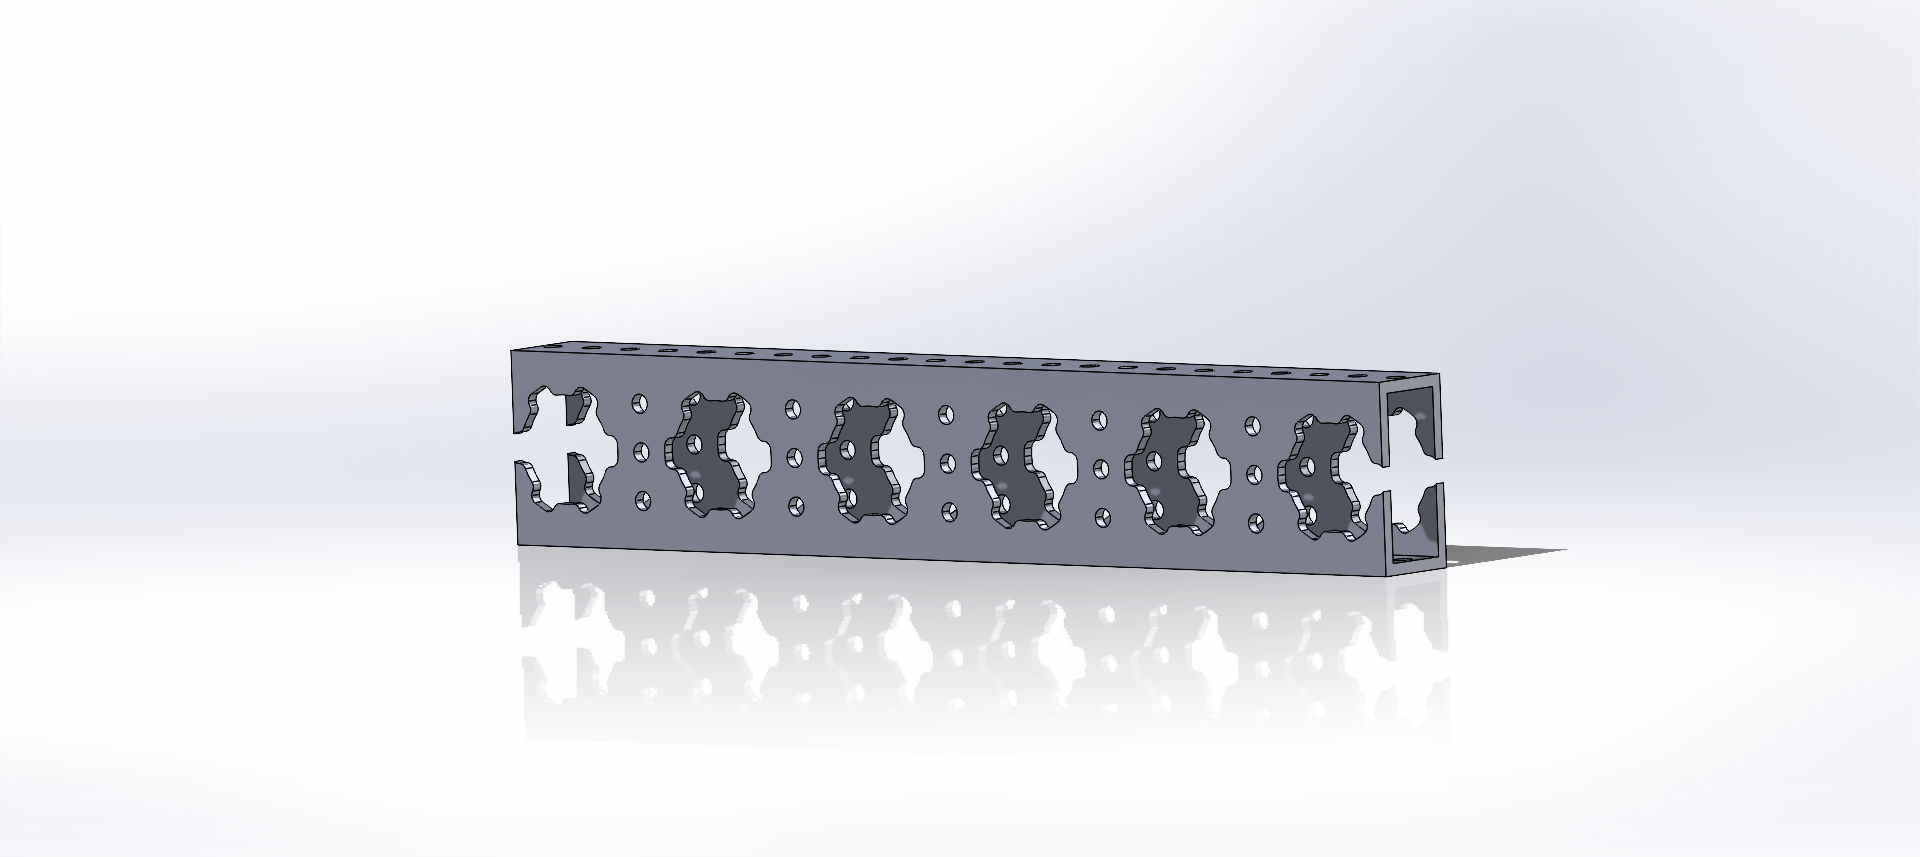
\includegraphics[width=0.49\textwidth]{media/MAXTube Cut.PNG}
\hfill
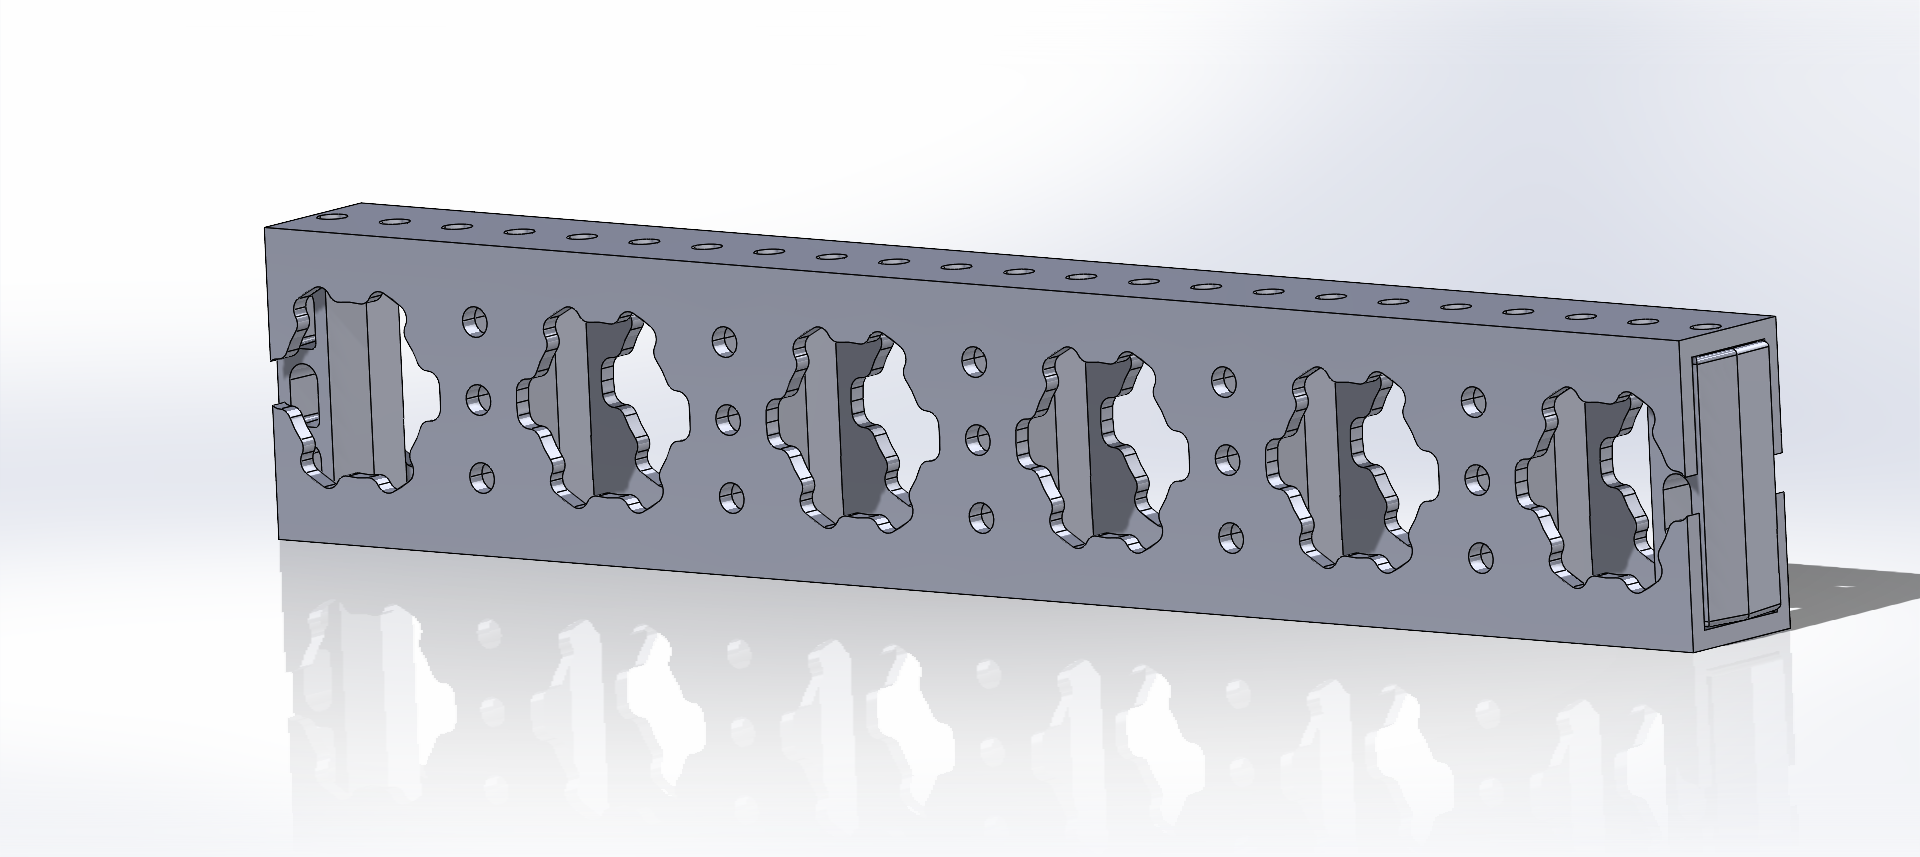
\includegraphics[width=0.49\textwidth]{media/MAXTubeAssem.PNG}

\caption{The cut 2×1 MAXTube with internal supports seated at each end and hole set.}
\end{figure}

\assemblystep{Build the Base Frame}
Place 3 T-Nuts in one side of 4 508mm extrusions. Add a
drop of Loctite to the end of 3 30mm screws and attach the 2x1 channel
using the center three sets of holes. Do not tighten until the base is
properly aligned. Repeat these steps 3 more times.

\begin{figure}[H]
\centering
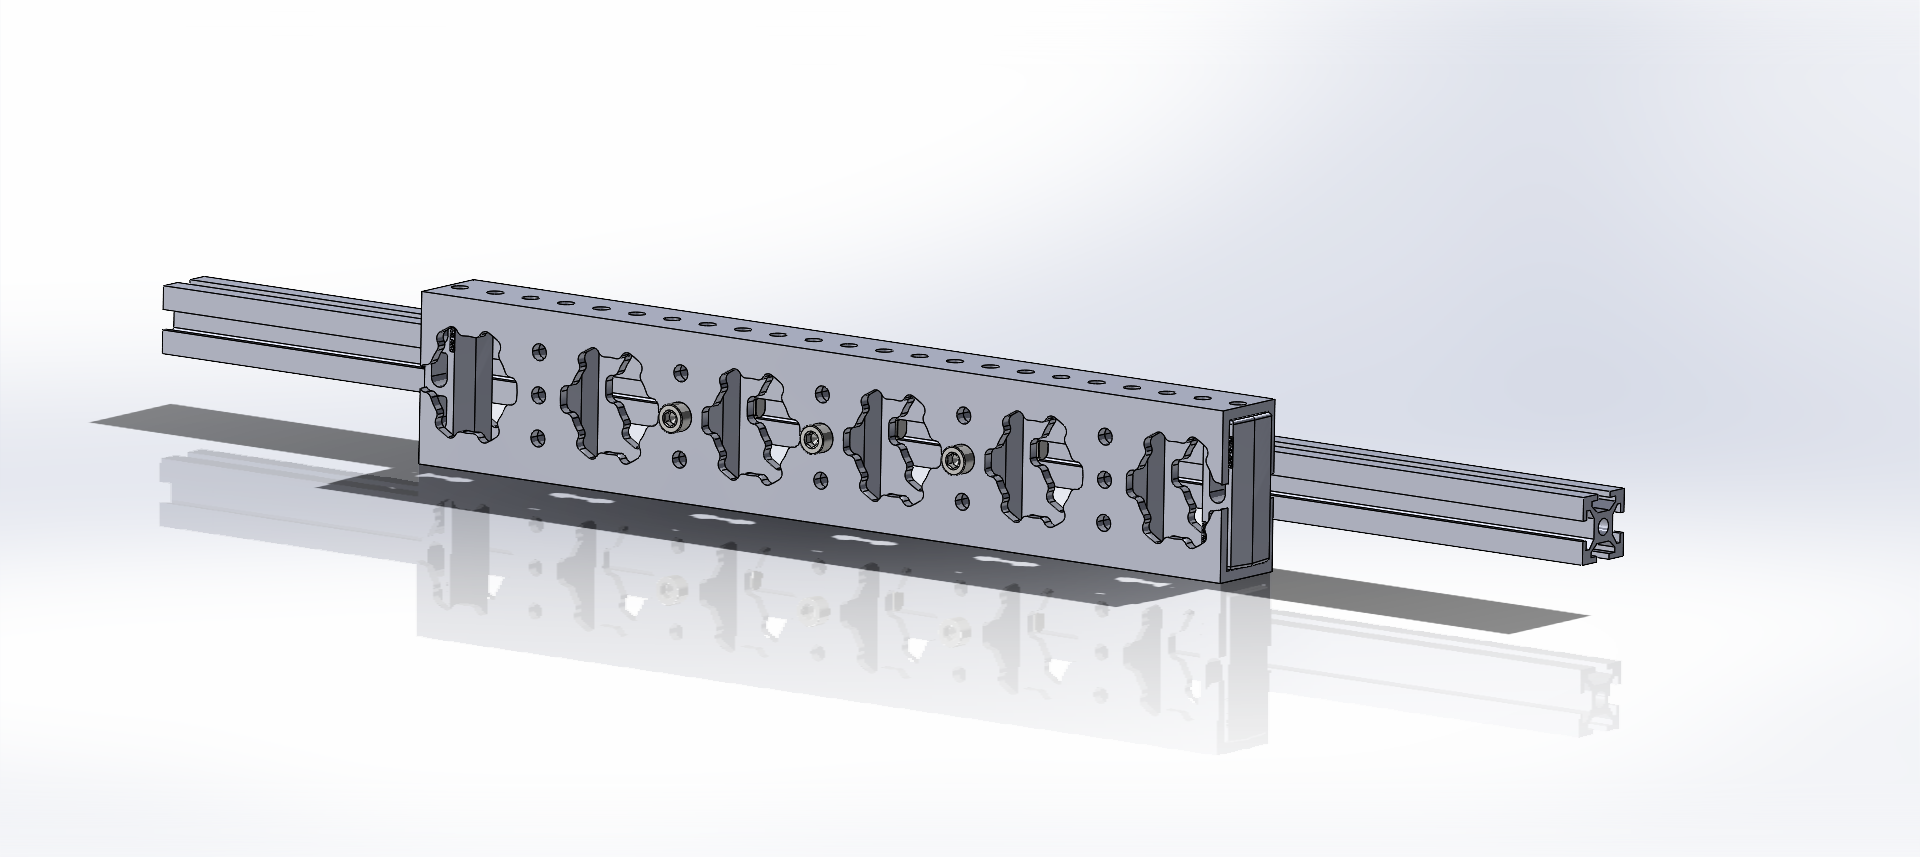
\includegraphics[width=0.5\textwidth]{media/MAXand510.PNG}
\caption{Attaching a 20x20mm extrusion to the 2x1 channel through the
center hole sets.}
\end{figure}

\assemblystep{Mount the Swerve Modules}
Remove the 2 long bolts on each side of the swerve modules and slide the
2x1 channel between the two plates. Secure with the bolts that were just
removed. Be sure to add Loctite to the ends of these bolts and secure
tightly. Repeat until the modules are assembled in a square. Add the
Tri-Connectors to the 20x20mm extrusions with the 2-pronged side facing
upwards.

\begin{figure}[H]
\centering
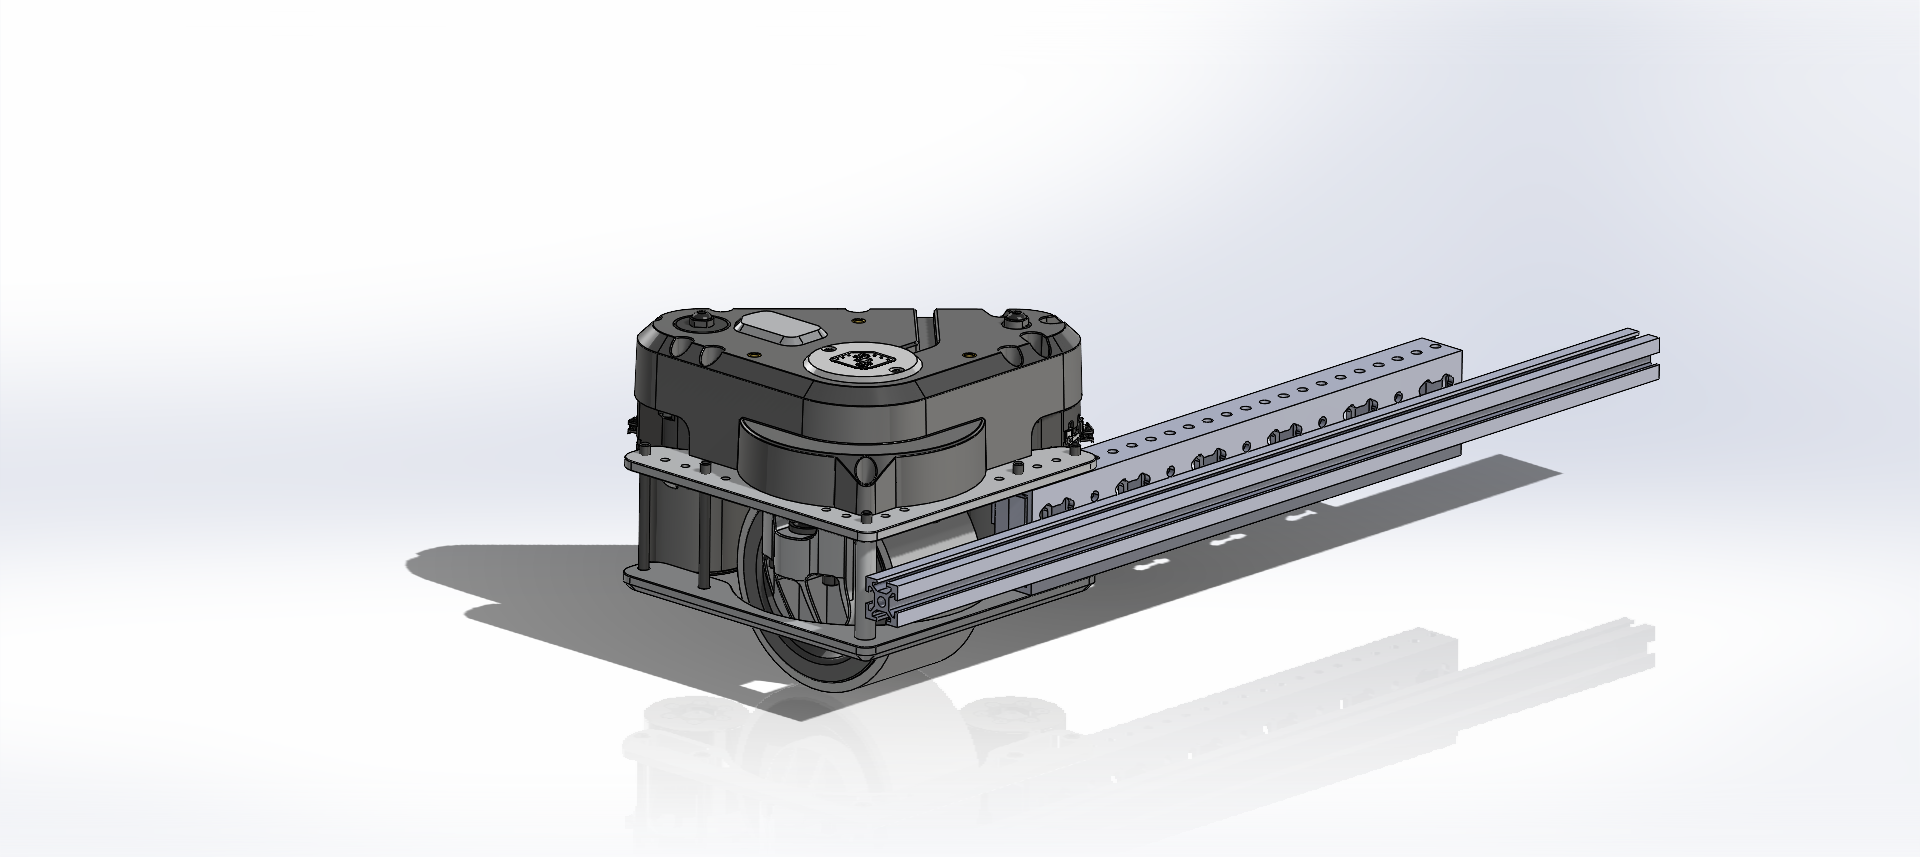
\includegraphics[width=0.6\textwidth]{media/SwerveAndMax.PNG}
\hfill
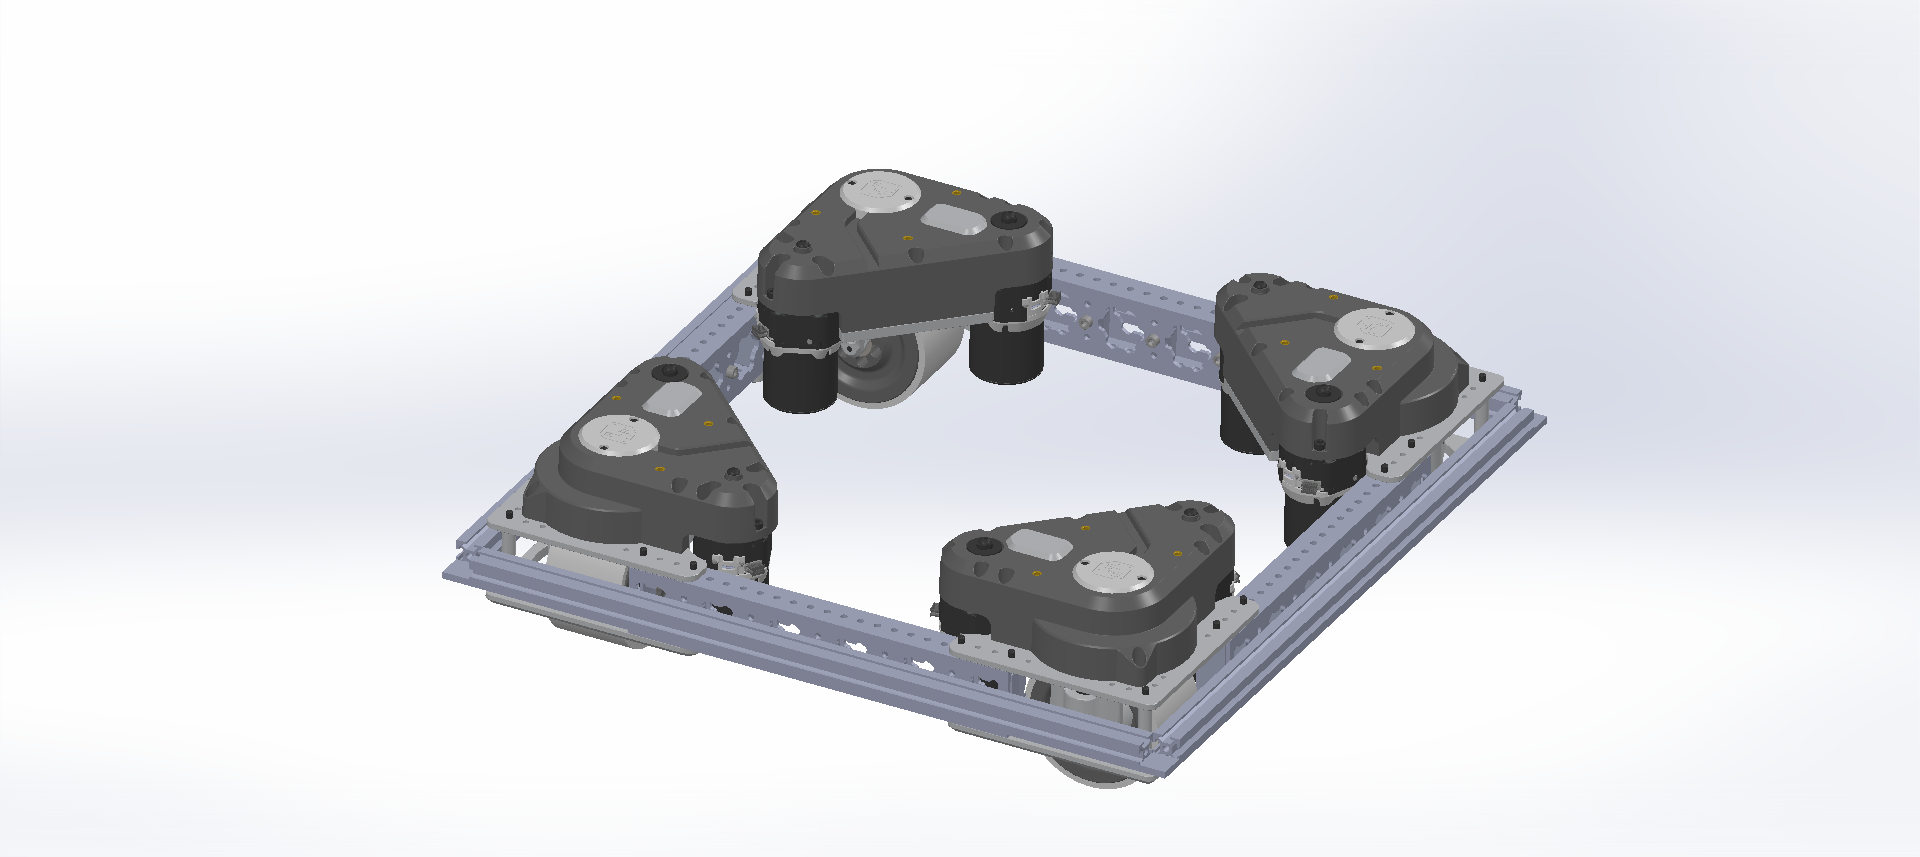
\includegraphics[width=0.6\textwidth]{media/SwerveSquare.SLDASM.PNG}
\caption{Sliding the 2x1 channels between the swerve module plates and
adding the Tri-Connectors.}
\end{figure}

\assemblystep{Install the Vertical Extrusions}
Vertically install 4 400mm extrusions, one at each corner. Tighten the set
screws.

\begin{figure}[H]
\centering
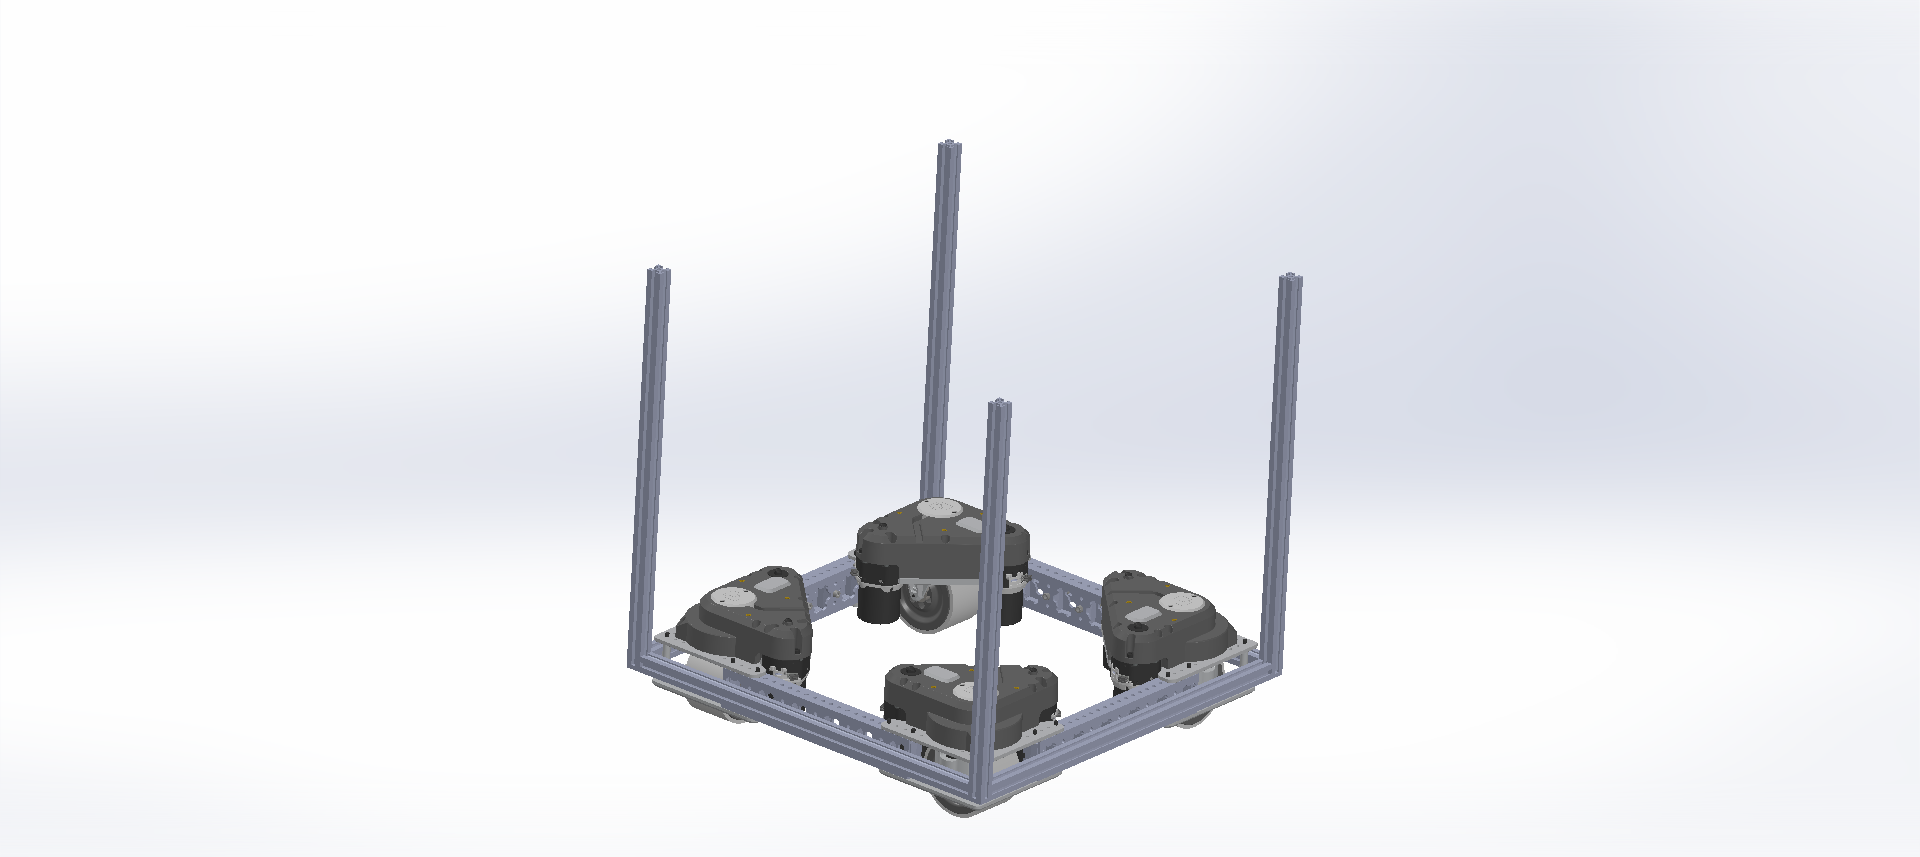
\includegraphics[width=0.75\textwidth]{media/BottomLayer.PNG}
\caption{A vertical 20x20mm extrusion installed at a corner via the
Tri-Connector.}
\end{figure}

Make sure the four extrusions are aligned properly and add the set pins
to the Tri-Connectors. Then tighten the M5x30mm bolts going through the
2x1'' channel.

\assemblystep{Install Corner Brackets}
Install a corner bracket at each 90 degree angle. Each one will use two
T-Nuts and two M5x8mm button head screws. Be sure to secure with
Loctite.

\begin{figure}[H]
\centering

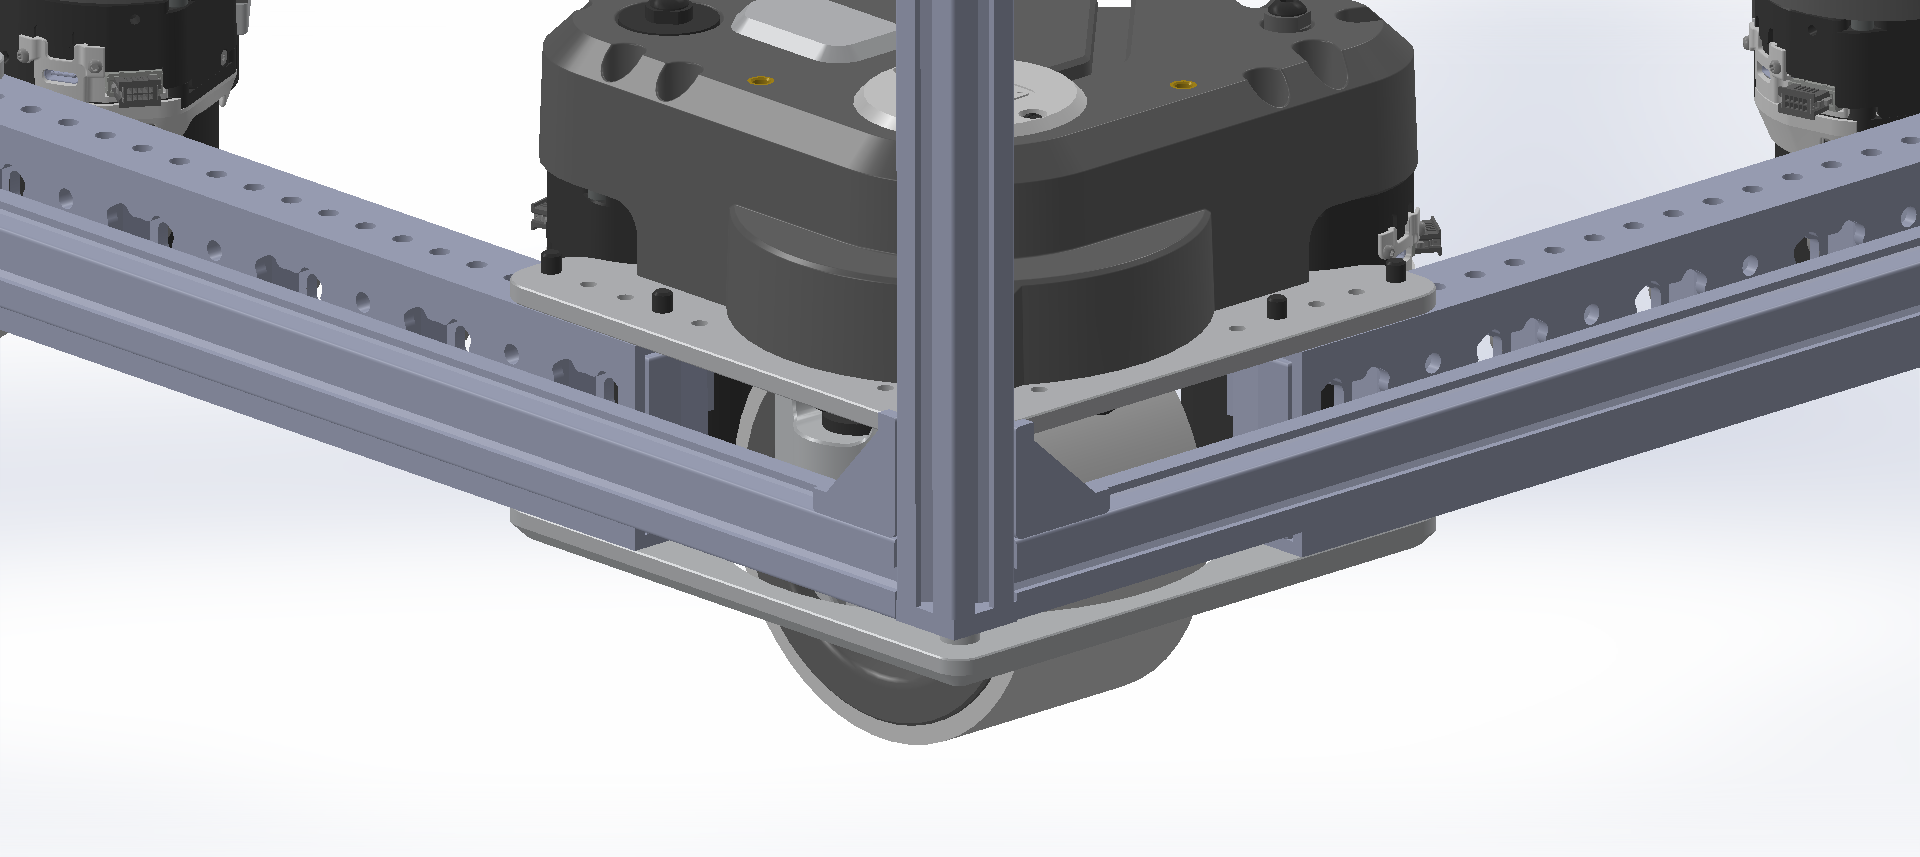
\includegraphics[width=0.75\textwidth]{media/BottomCB.PNG}
\caption{A corner bracket installed at a 90$^\circ$ joint with two T-Nuts
and two button head screws.}
\end{figure}

\assemblystep{Install L-Shape Corner Plates}
Install a L-shape corner plate at each of these locations using 4 T-Nuts
and 4 M5x8mm button head screws. Do not tighten until all 4 screws are
in place. Be sure to secure with Loctite.

\begin{figure}[H]
\centering
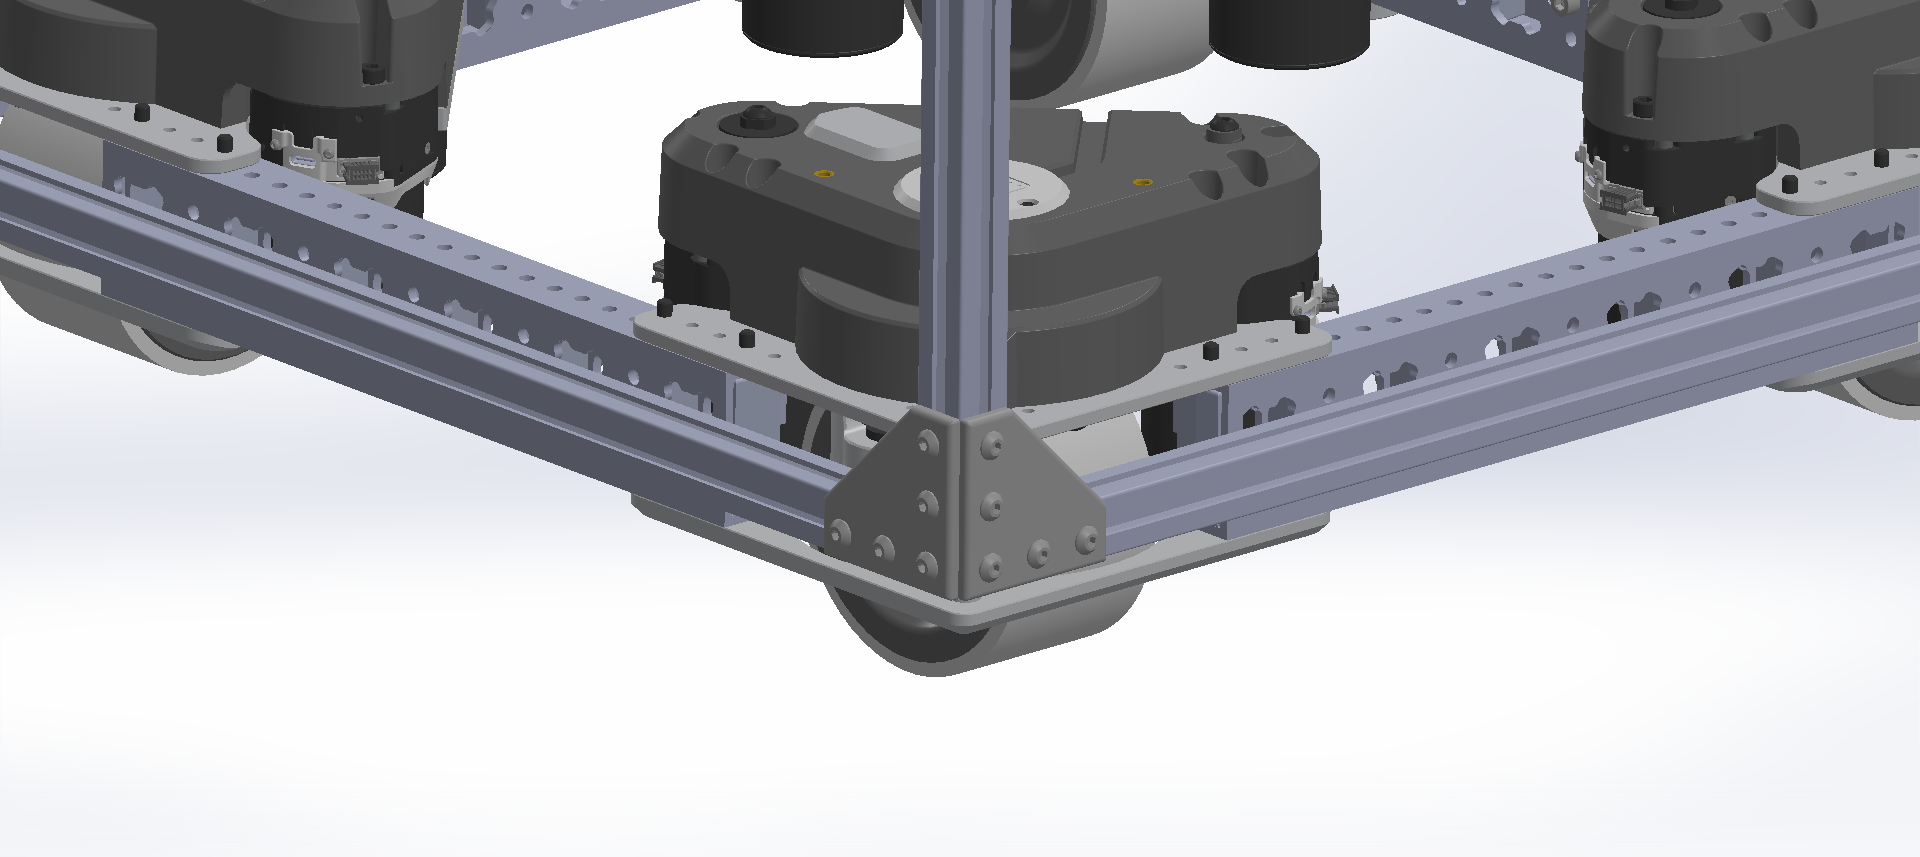
\includegraphics[width=0.75\textwidth]{media/BottomCP.PNG}

\caption{An L-shape corner plate fastened with four T-Nuts and four
button head screws.}
\end{figure}

\assemblystep{Add the Underside Extrusions}
Affix two pieces of 20x20x508 extrusions to the underside of the base
using a T-Nut and a M5x50mm socket head screw on each end. Use the
mounting holes on the inner side of the internal supports of the 2x1"
channels as shown below. Be sure to secure with Loctite.

\begin{figure}[H]
\centering
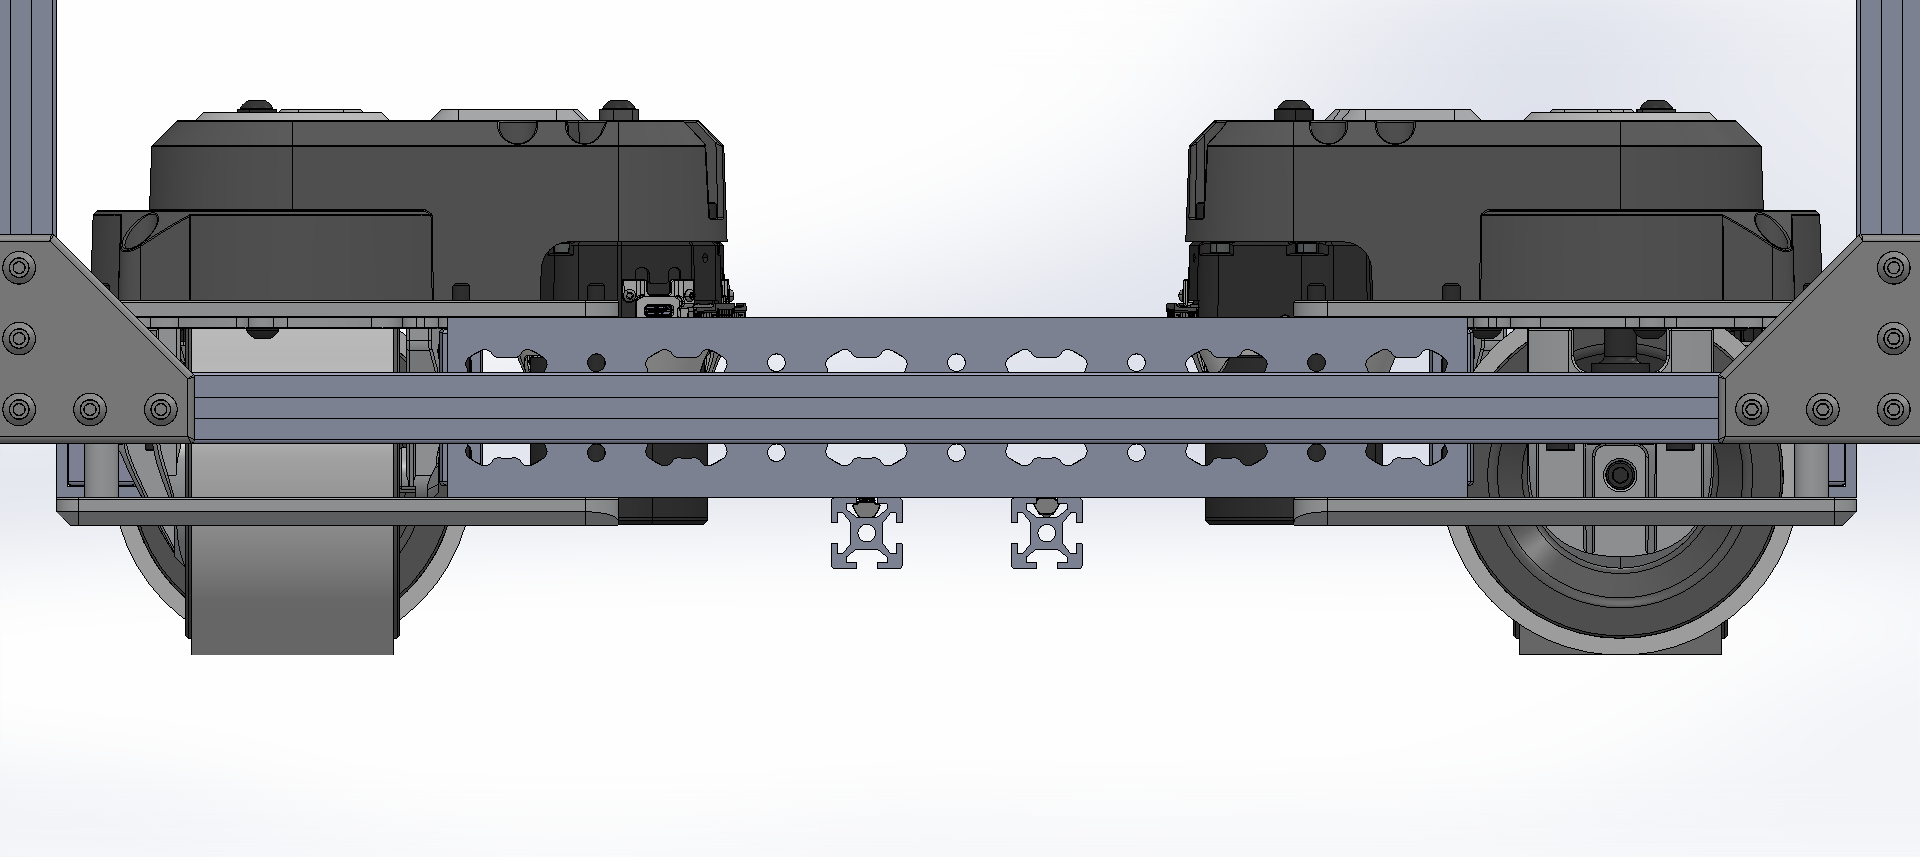
\includegraphics[width=0.47\textwidth]{media/BottomRails.PNG}
\hfill
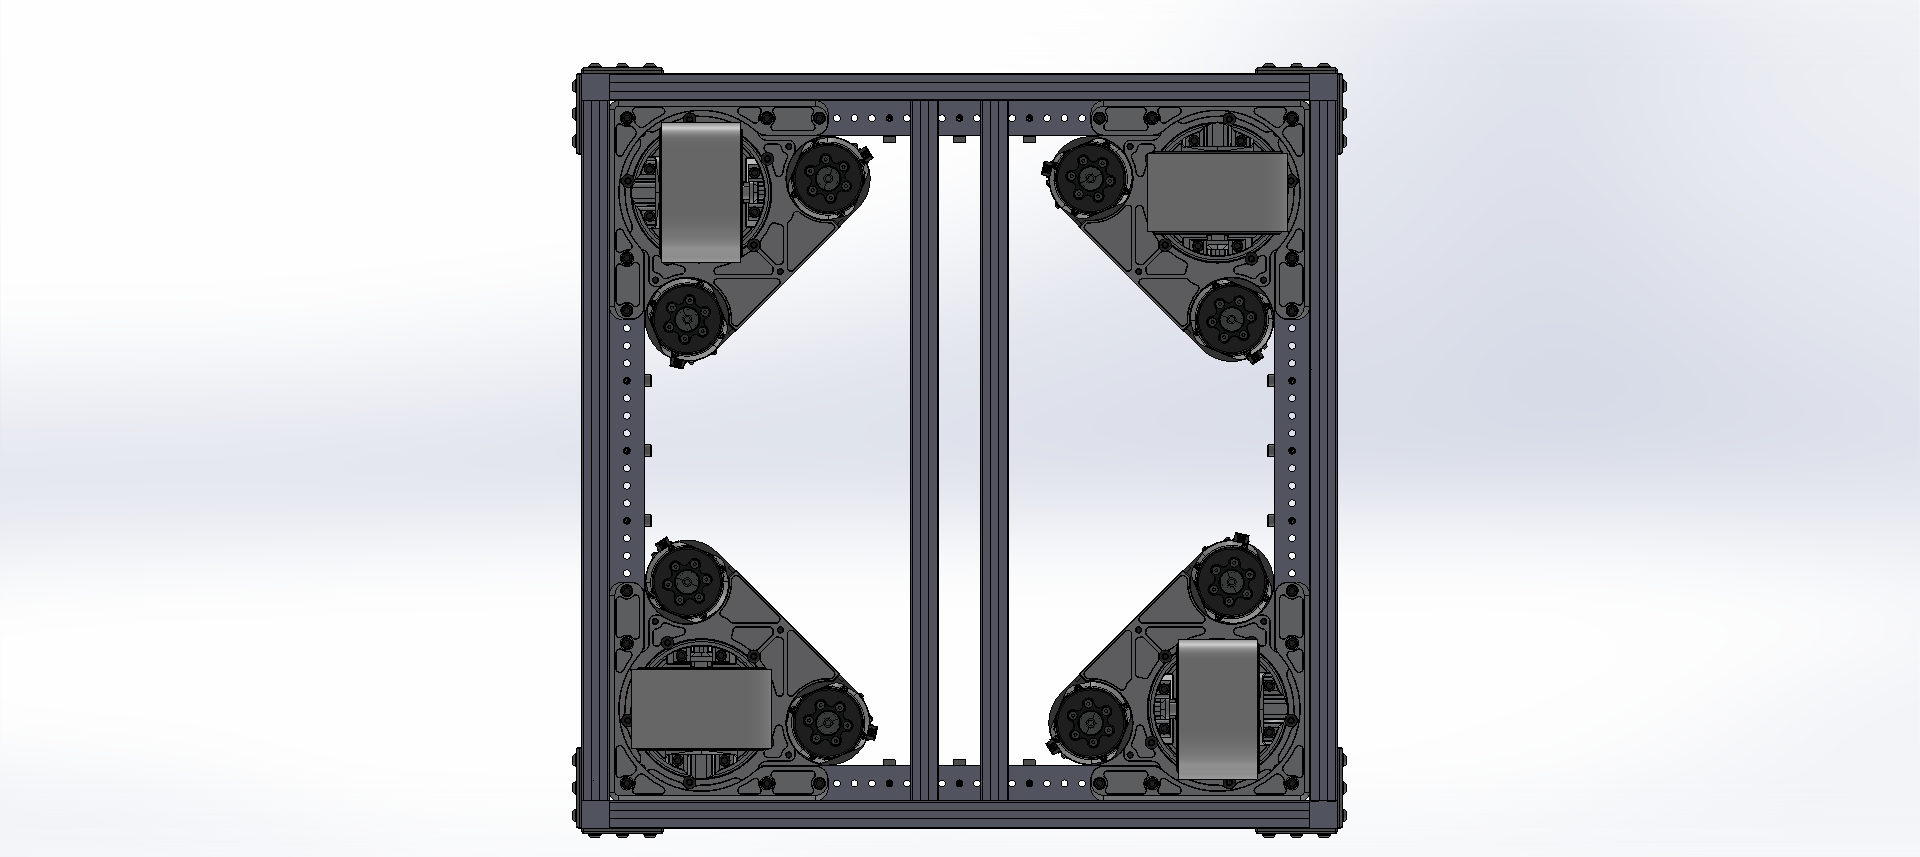
\includegraphics[width=0.47\textwidth]{media/BottomRails1.PNG}
\caption{Two 20x20x508 extrusions affixed to the underside of the base
along the internal supports.}
\end{figure}

\assemblystep{Build the Control Box Mounts}
Cut a piece of 3x1 inch linear rail to 5" and a piece of the 2x1"
channel to 3". Use two M5x16mm bolts, washers, and nuts to secure the
channel to top of the existing channel on one of the sides that the
bottom two 20x20mm extrusions are not mounted to. 
Secure the linear rail to the top of the channel with two M5x10mm bolts, washers, and nuts. Be sure to secure with Loctite.


\begin{figure}[H]
\centering
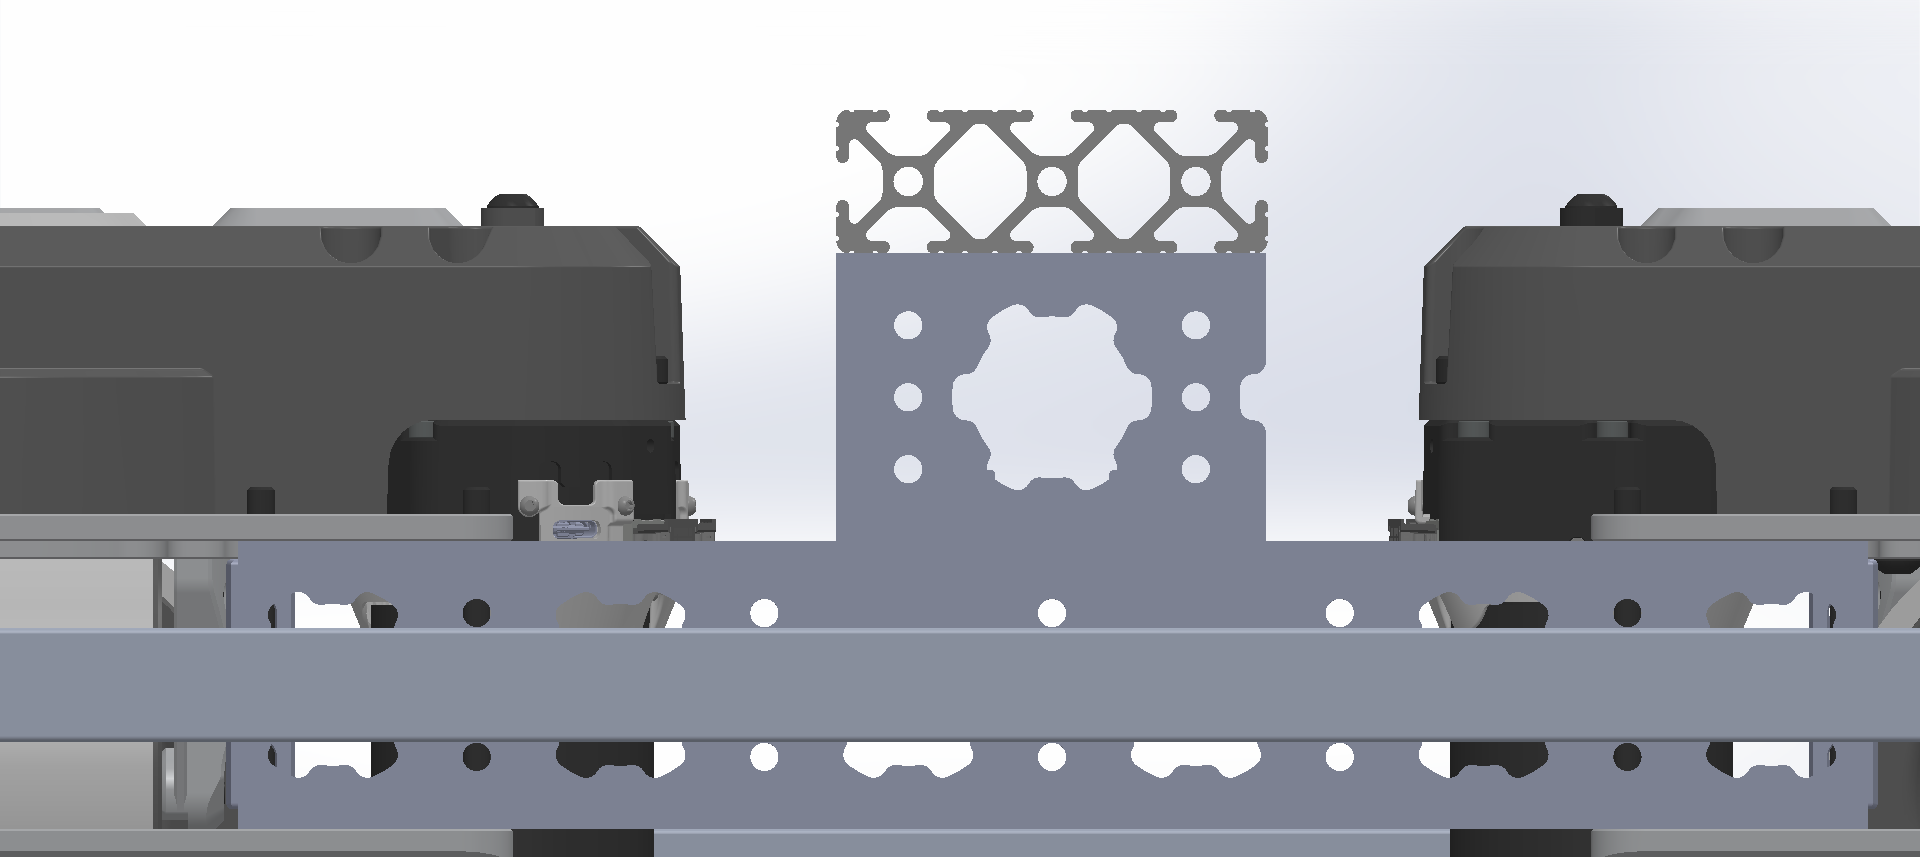
\includegraphics[width=0.47\textwidth]{media/CBMountSide.PNG}
\hfill
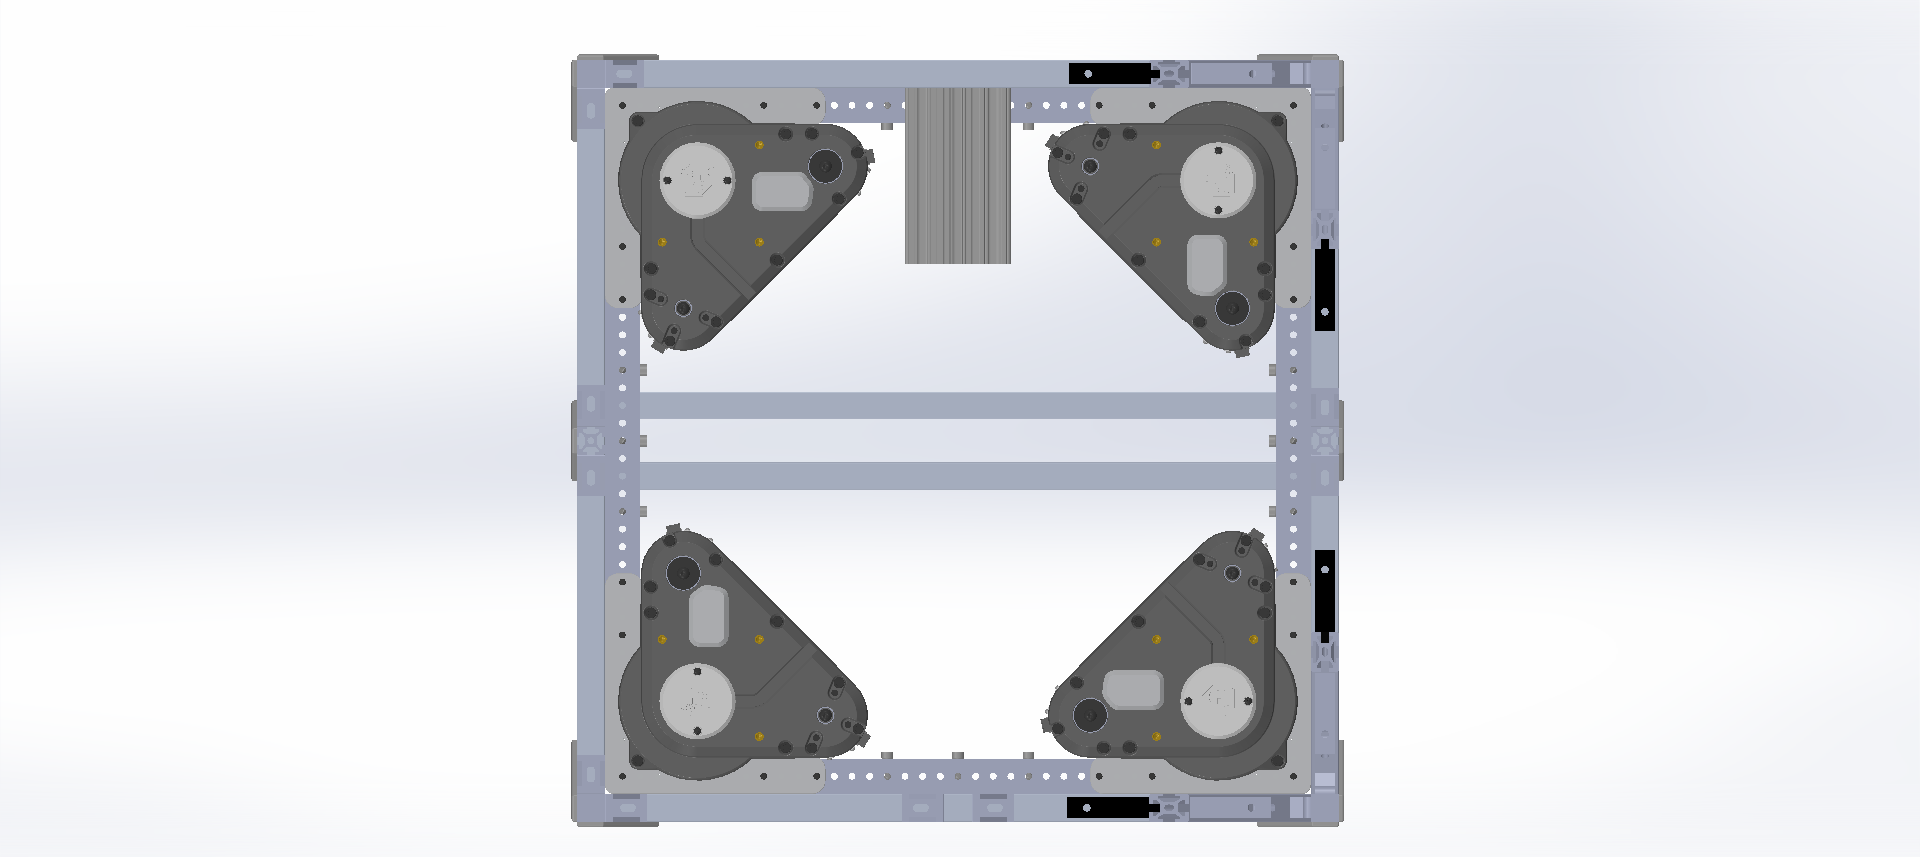
\includegraphics[width=0.47\textwidth]{media/CBMountTop.PNG}
\caption{Control box mount.}
\end{figure}

\assemblystep{Mount the Battery}
Place the Anker battery in the center of the base along the extrusions.
Affix using the ratcheting rope hangers by wrapping the non-ratchet end
around a extrusion and clipping the carabiner to the rope. Feed the
other end around both extrusions, then up to the battery handle. Wrap
around the handle twice before bringing the ratchet down and clipping to
the first carabiner. Pull the excess rope until tight and tie a knot a
few inches away from the ratchet. Cut the excess.

\begin{figure}[H]
\centering
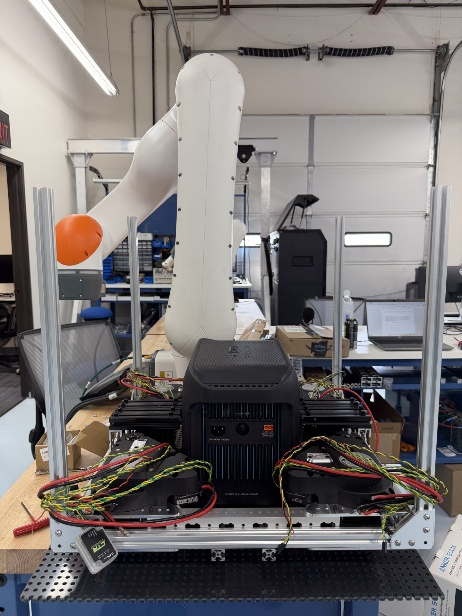
\includegraphics[width=0.23\textwidth]{media/image78.jpeg}
\hfill
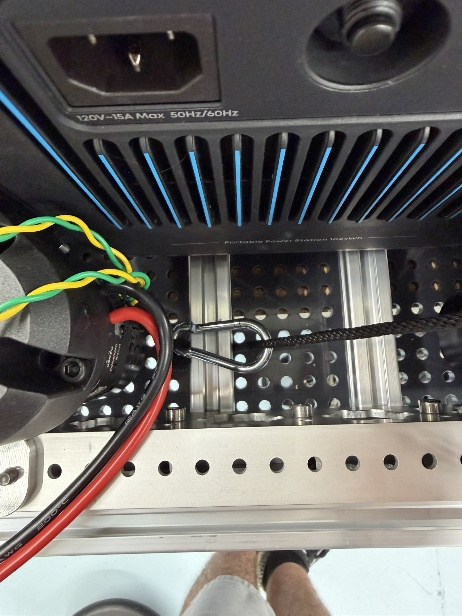
\includegraphics[width=0.23\textwidth]{media/image79.jpeg}
\hfill
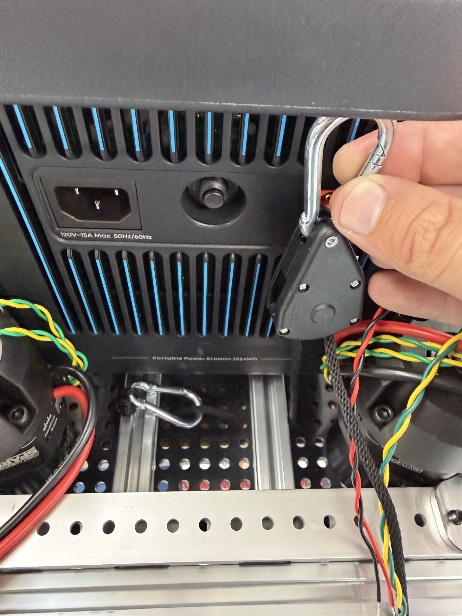
\includegraphics[width=0.23\textwidth]{media/image80.jpeg}
\hfill
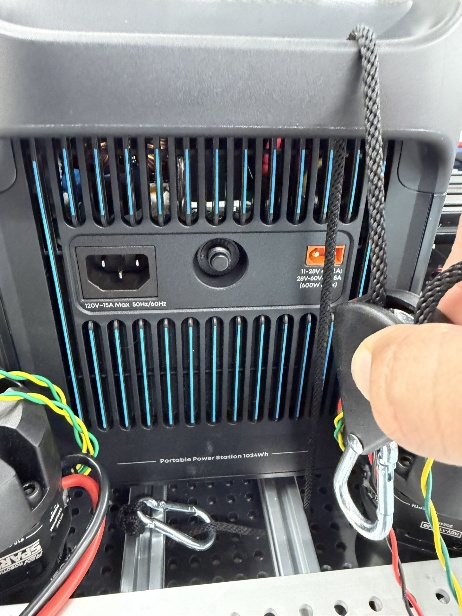
\includegraphics[width=0.23\textwidth]{media/image81.jpeg}

\vspace{0.4cm}
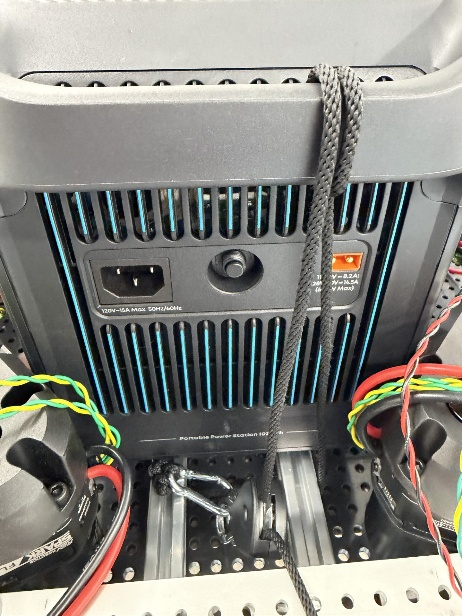
\includegraphics[width=0.23\textwidth]{media/image82.jpeg}
\hfill
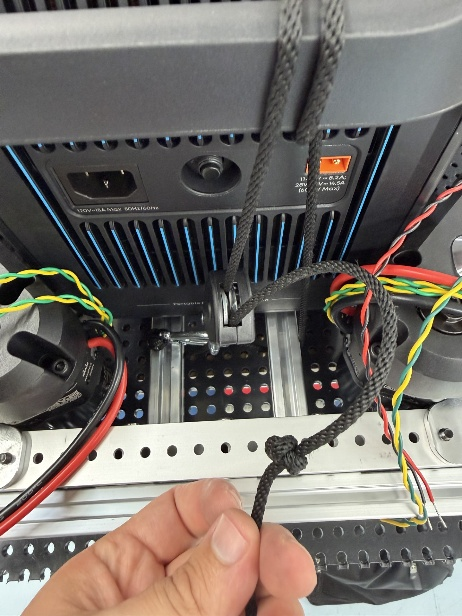
\includegraphics[width=0.23\textwidth]{media/image83.jpeg}
\hfill
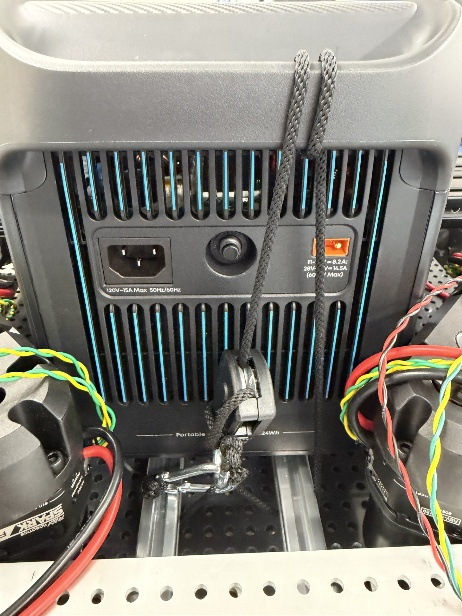
\includegraphics[width=0.23\textwidth]{media/image84.jpeg}
\hfill
\hspace{0.23\textwidth}
\caption{Securing the Anker battery to the base with ratcheting rope
hangers.}
\end{figure}

\assemblystep{Route and Solder the Signal Wires}
Starting with the encoder that has the CANivore, take the other set of
signal wires and daisy-chain them to the next encoder. Repeat until the
4 encoders are in series. Repeat these steps with all motor signal wires
as well. Next, trim the wires to take the slack out and solder them
together. Do not forget to add shrink wrap to prevent shorts in exposed
wires. Leave enough slack for adequate cable management. Use zip ties to
attach to frame. It may be useful to remove the battery, but make sure
cables will not be pulled by battery upon reinstallation.

\begin{figure}[H]
\centering
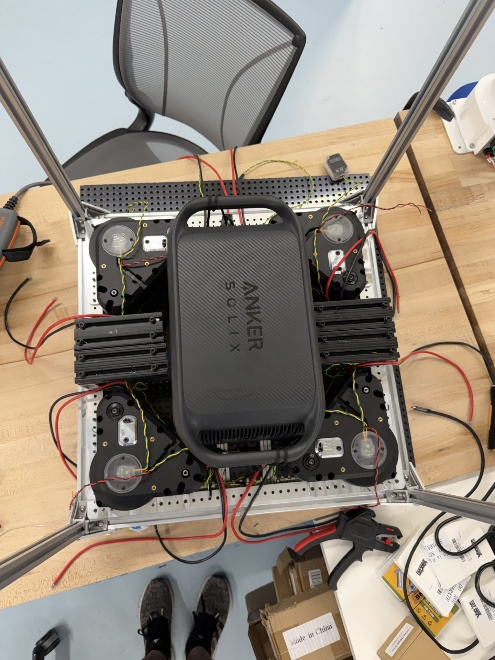
\includegraphics[width=0.47\textwidth]{media/image85.jpeg}
\hfill
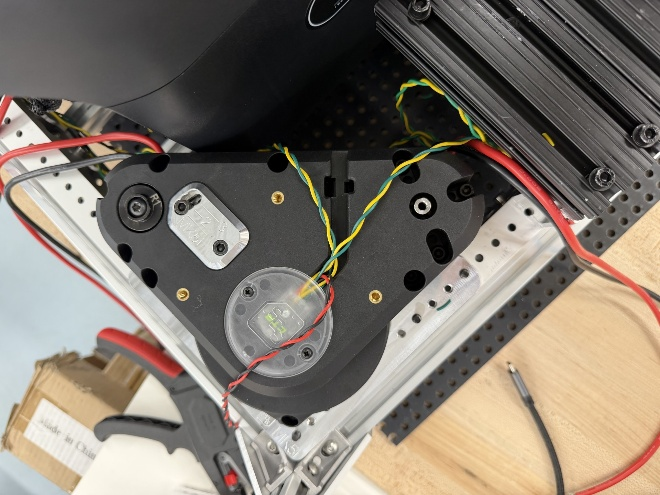
\includegraphics[width=0.47\textwidth]{media/image86.jpeg}
\caption{Daisy-chaining, trimming, and soldering the encoder and motor
signal wires with shrink wrap.}
\end{figure}

\assemblystep{Install the Lower Control Box}
Place the XArm 850 A/C control box on each control box stand. Be sure that the
emergency stop is facing upwards and the power switch is facing the
side designated as the front. The handle may need to be removed from the
unit. Affix with a double-sided adhesive, such as Velcro.

\begin{figure}[H]
\centering
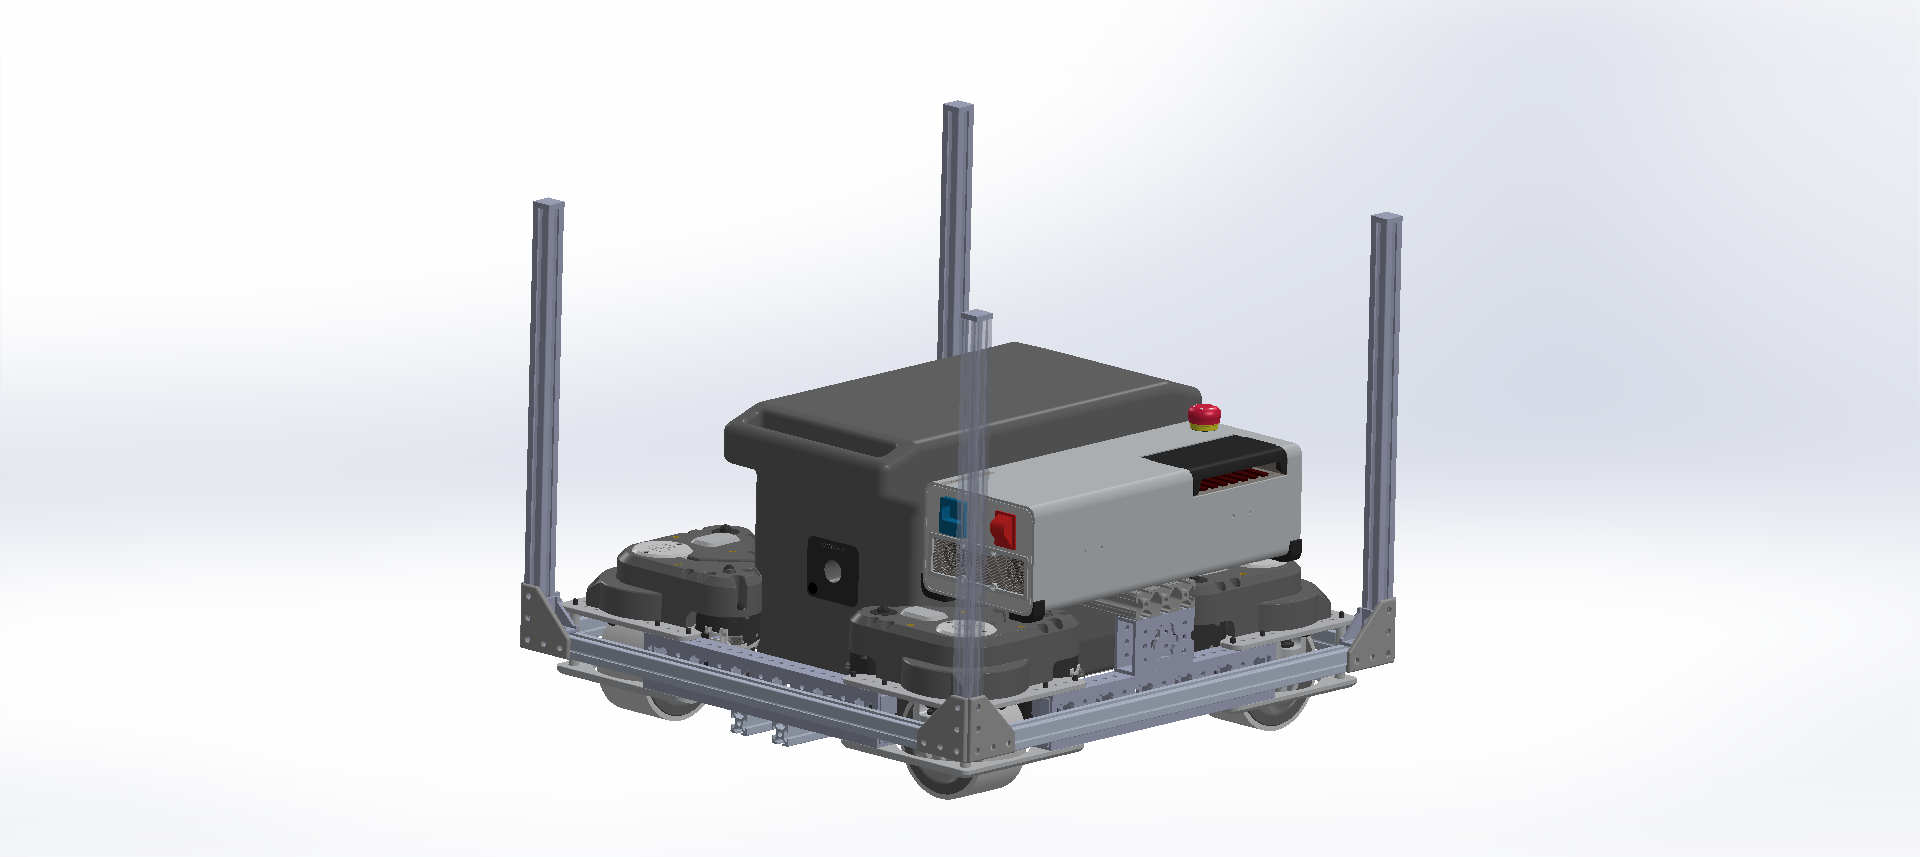
\includegraphics[width=0.75\textwidth]{media/CBInstalled.PNG}

\caption{An A/C control box mounted on its stand with the emergency stop
facing upwards.}
\end{figure}

\assemblystep{Install Vertical Bracing to Middle Layer}
Install 4 20x20x205mm vertically on the center of each side of the horizontal extrusions using 2 corner brackets, 4 T-Nuts, and 4 M5x8mm button head screws on each extrusion. Be sure to secure with Loctite.
Then, install a T-Plate over each joint using 4 T-Nuts and 4 M5x8mm button head screws. Be sure to secure with Loctite.

\begin{figure}[H]
\centering
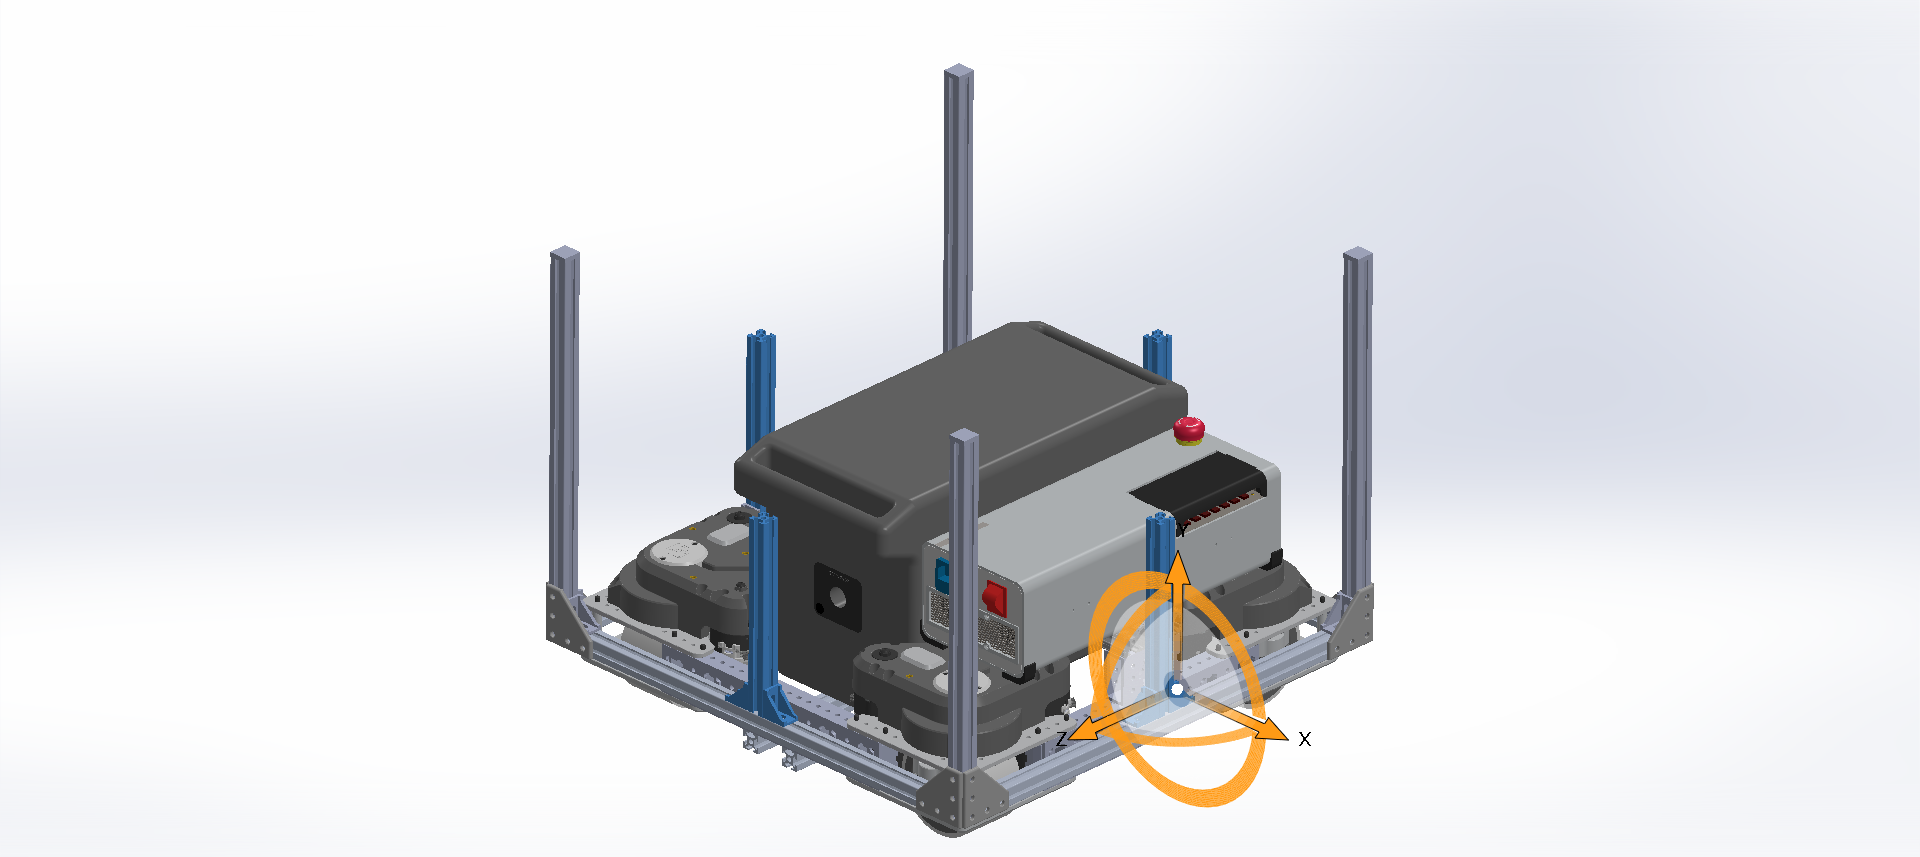
\includegraphics[width=0.47\textwidth]{media/BotVertSup.PNG}
\hfill
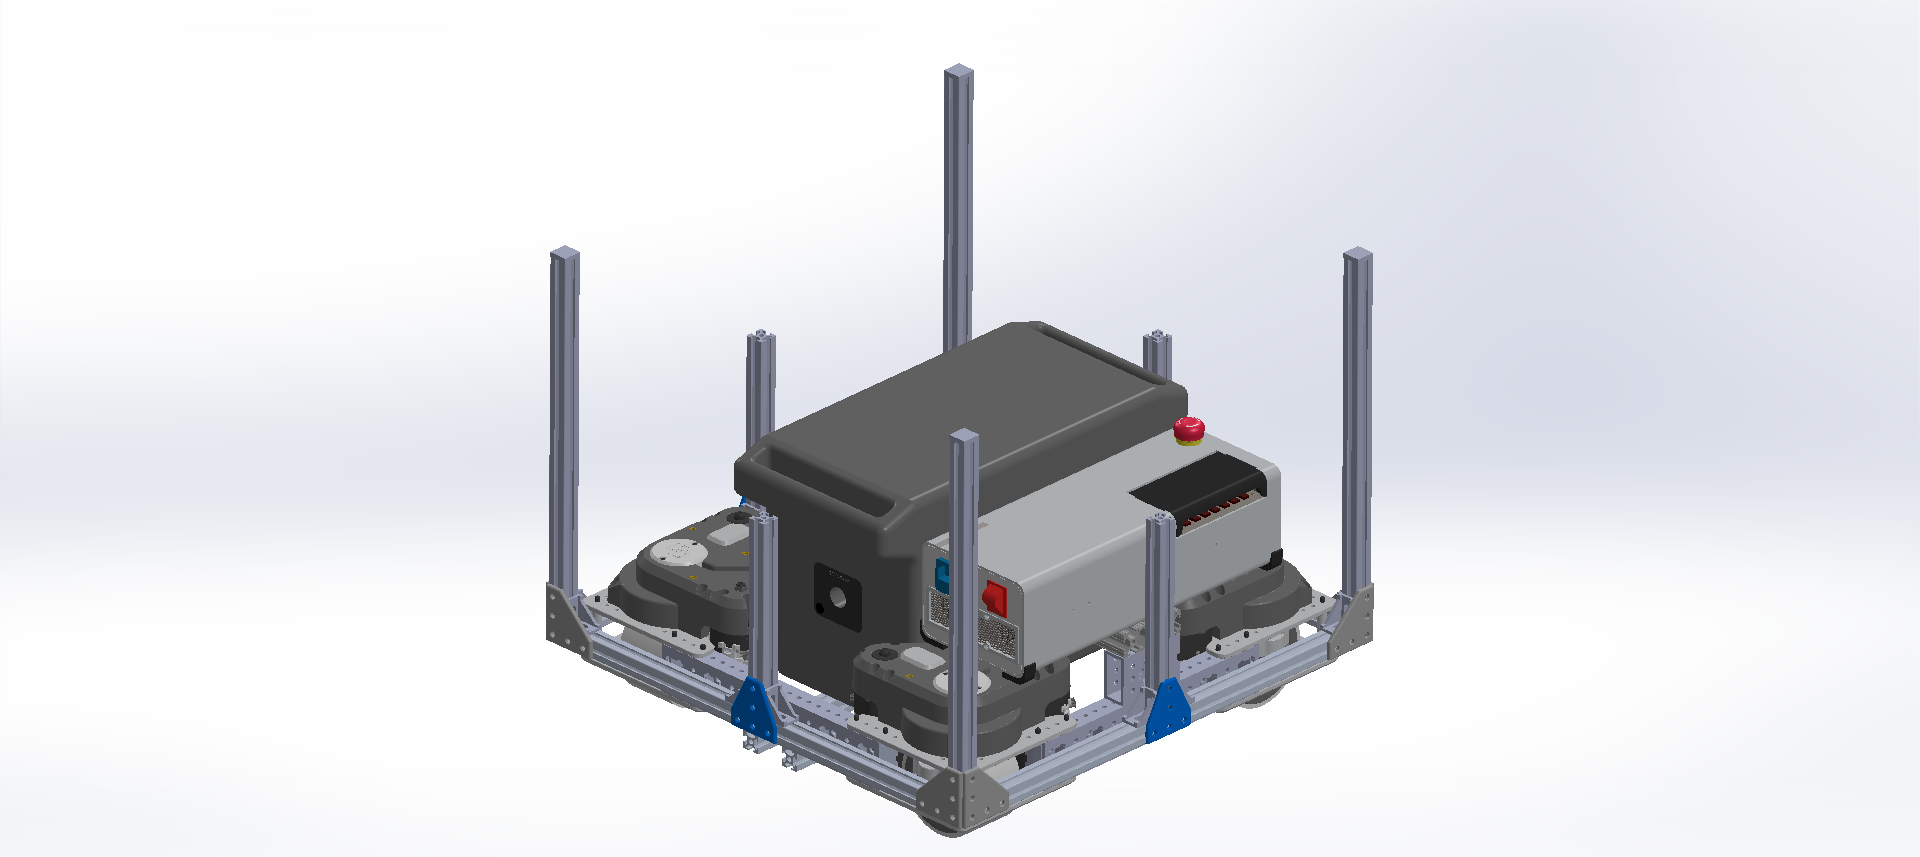
\includegraphics[width=0.47\textwidth]{media/BotTPlate.PNG}
\caption{Vertical bracing and T-plates installed on the center of each
side of the horizontal extrusions.}
\end{figure}

\assemblystep{Install Angled Bracing to Middle Layer}
Install a 135\textdegree angle bracket on each side of the two front corners using a T-Nut and a M5x10mm button head screw. One end should be coincident with the corner bracket.
Install a trapezoidal shaped brace with the longest edge being 164mm above the 135\textdegree angle bracket with another T-Nut and M5x10mm button head screw.
Install a 45\textdegree angle bracket connecting the brace to the vertical extrusion with a T-Nut and M5x10mm button head screw.
Install another 45\textdegree angle bracket with one side aligned with the upward facing side of the brace and extending towards the corner. Use a T-Nut and M5x10mm button head screw.
Be sure to secure with Loctite.

\begin{figure}[H]
  \centering
  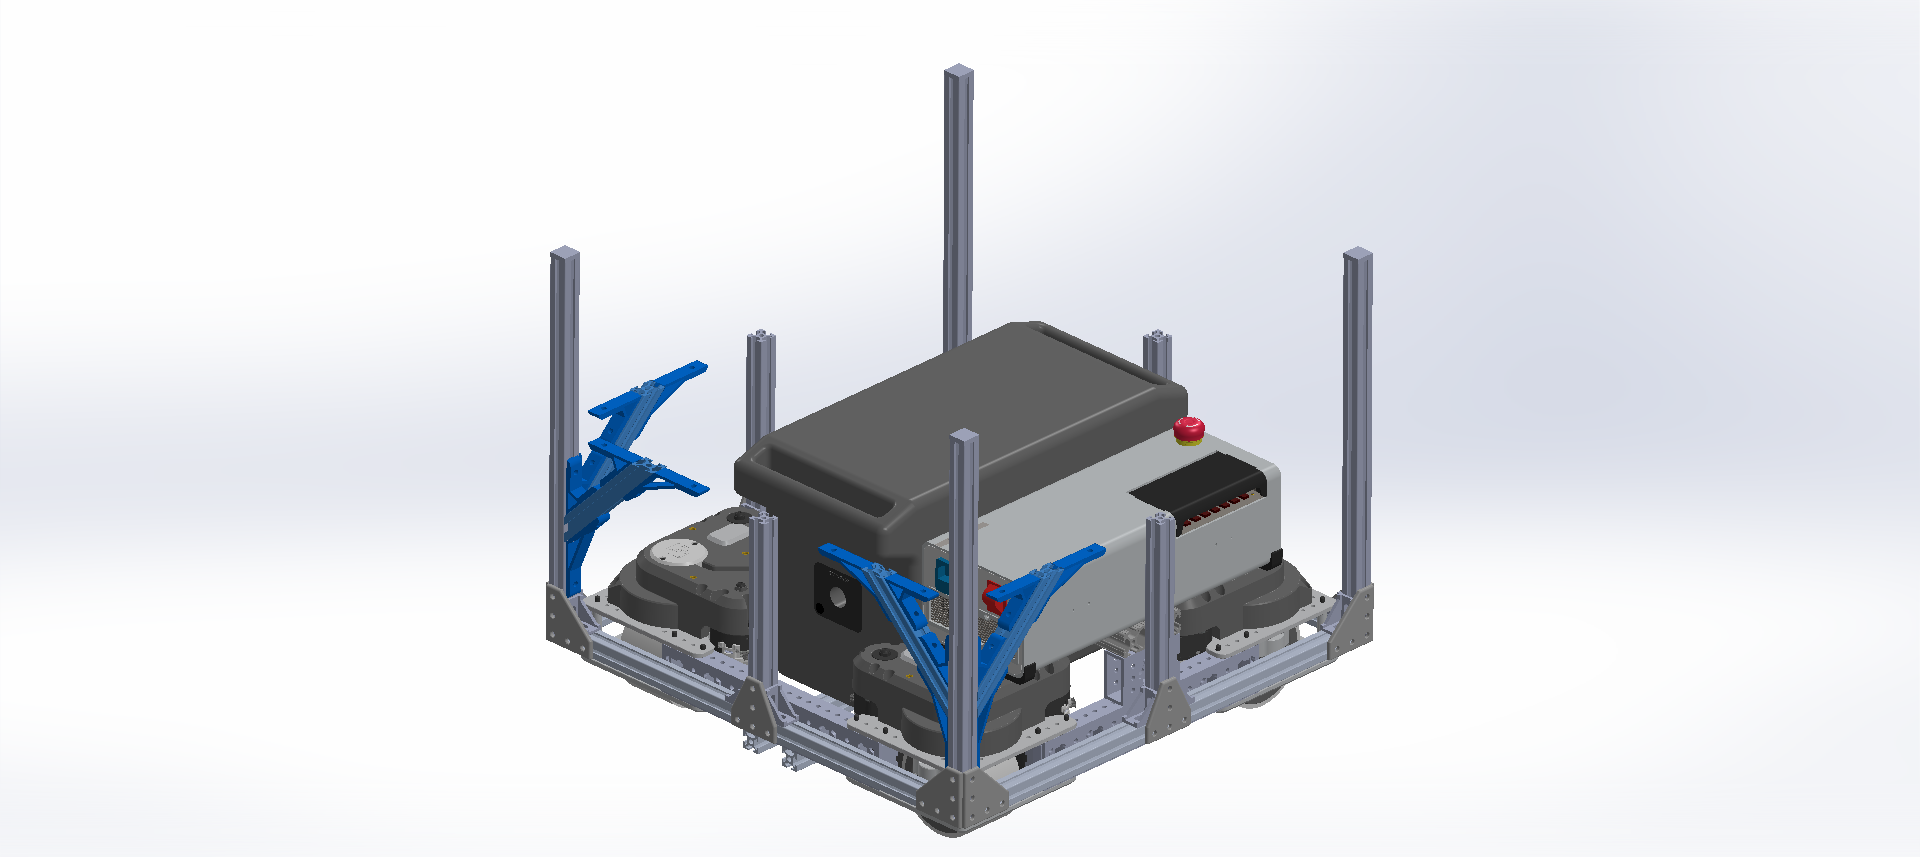
\includegraphics[width=0.75\textwidth]{media/BotAngleBraces.PNG}

  \caption{The angled support braces installed.}
\end{figure}